%********************************************************************
% --------- Document Preamble
% *******************************************************************
\documentclass[a4paper,12pt]{article}

% used packages:
\usepackage{amsmath, amssymb, latexsym, amscd, amsthm,amsfonts,amstext}
\usepackage[mathscr]{eucal}
\usepackage{graphicx}
\usepackage{subfigure}


% Specify the page layout:
\textwidth = 15cm
\textheight = 22.5cm
\topmargin = 0cm
\headsep =20pt
\oddsidemargin = 15pt
\evensidemargin = -15pt

\renewcommand{\baselinestretch}{1.1} % stretch the ver. space between 2 lines

% --------- Mathematical specification:
\newtheorem{theorem}{Theorem}[section]
\newtheorem{lemma}[theorem]{Lemma}
\newtheorem{definition}[theorem]{Definition}
\newtheorem{algorithm}[theorem]{Algorithm}

\def\bR{\mbox{\boldmath$R$}}

\pagestyle{myheadings}
% *********************************************************************
% End of document Preamble
% *********************************************************************


%opening
\title{Pre-processing of UNCC experimental backscattering data}
\author{Nguyen Trung Th\`anh\footnote{Need help? You can email me at \texttt{nguyen.trung.thanh.1979@gmail.com}}} 



\begin{document}

\maketitle

\noindent\textbf{Updates in version 3}

\begin{itemize}
 \item Add data preprocessing steps for frequency domain data in 2016. 

\end{itemize}

\section{Time-depedent data}
This type of data was measured at the UNCC in 2012 - 2014. 

\subsection{Data acquisition and data structure}

\subsubsection{Some terms used in this document}
\begin{itemize}
\item \textit{Experiment}: One experiment is a data acquisition which usually contains a number of data files, e.g., the incident wave file, the data set without target, the data sets containing targets. Data of each experiment is stored in a MAIN folder. For example, in the folder ``examples'', there are two experiments: ``dataset\_air'' and ``data\_sandbox''. You can choose an arbitrary name you want.  

\item \textit{Data set}: this term is used for a specific data file of ONE measurement (scan).  
Each data set of an experiment is stored in a subfolder of the MAIN folder of that experiment. 
This subfolder is usually named ``object\_n'', where n can be 1, 2, etc. See ``dataset\_air'' or ``data\_sandbox'' for the naming. However, you can also choose another naming style. However, the postfix ``\_n'' should be followed for automatic preprocessing. 

\item \textit{Target}: a target is a particular object placed in measurement. There may be no target, one target or more in each data set.
\end{itemize}

\subsubsection{Data acquisition}

Our experimental configuration is shown in Figure~\ref{fig:setup}. A horn antenna (transmitter) is fixed at a given
position and a detector is scanned row-by-row in a square of a vertical plane, which we
refer to as the measurement plane. Consider the Cartesian coordinate system $%
Oxyz$ as shown in Figure \ref{fig:setup}(b). The scanning area is 1 m by 1
m with the step size of 0.02 m, starting at $(x,y)=(-0.5,-0.5)$ (the top-left corner) and ending at 
$(x,y)=(0.5,0.5)$ (the bottom-right corner). \textbf{Note that the $y$-coordinate is looking downwards since the scanning starts from the top}. 

\textbf{Therefore, when the FEM grids are created for the forward solver of WaveES, the coordinate system should be the same as here. However, when the final results are visualized using AVS-Viewer, the images should be turned upside down.}

\begin{figure}[tph]
\centering
\subfigure[]{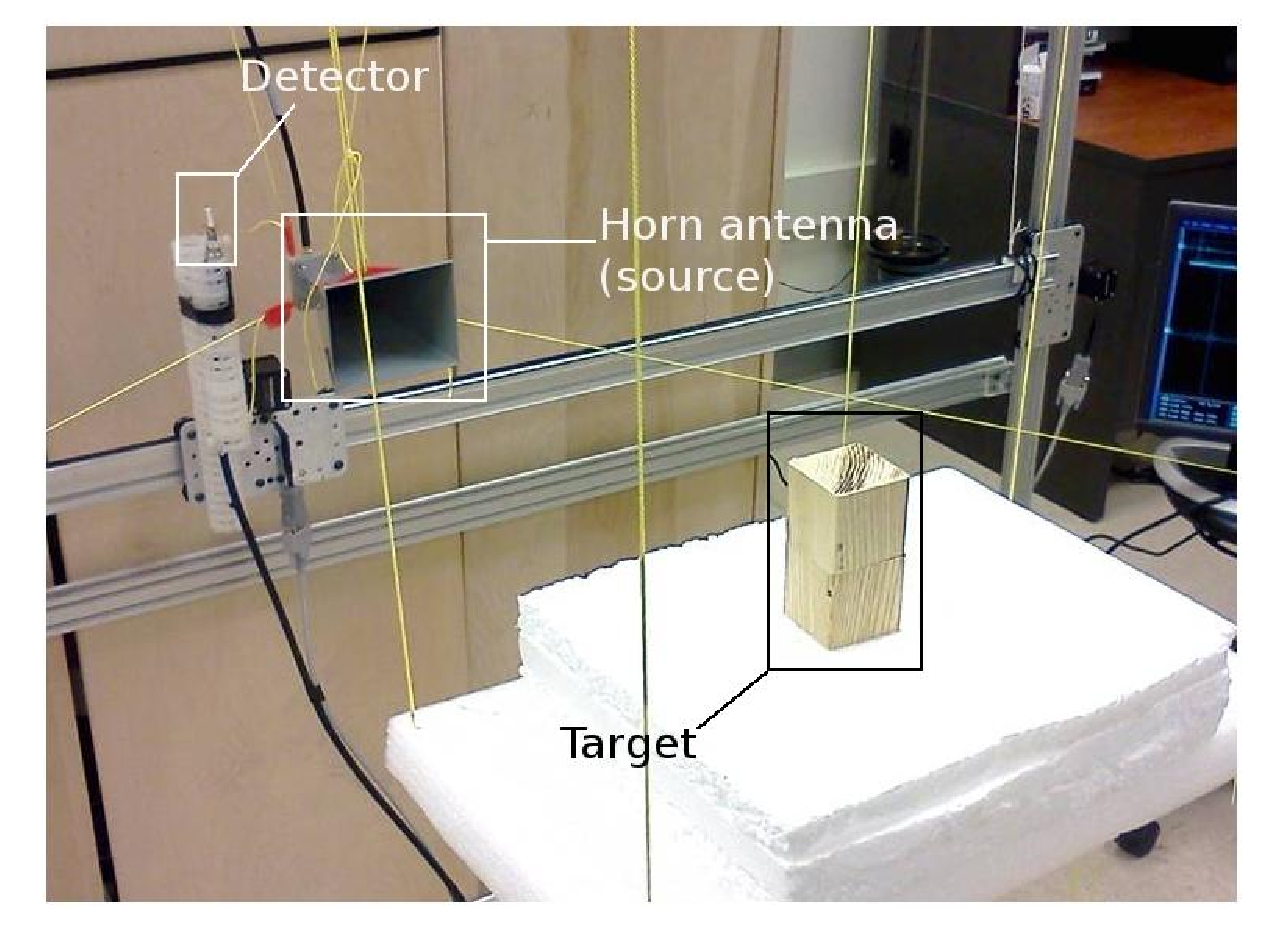
\includegraphics[width = 0.4\textwidth,height=0.3\textwidth]{figure/fig1a}} \hspace{%
0.3truecm} 
\subfigure[]{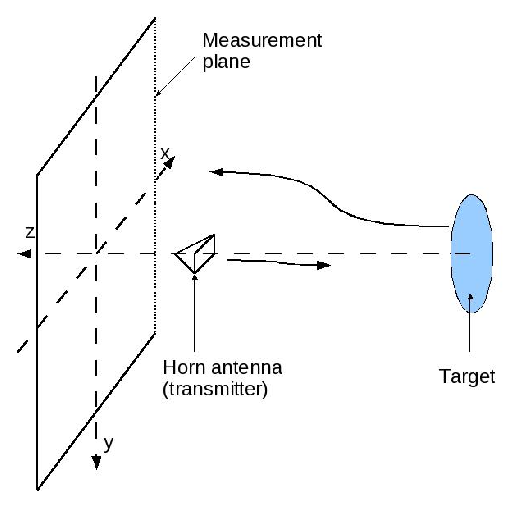
\includegraphics[width =
0.34\textwidth,height=0.3\textwidth]{figure/fig1b}}
\caption{(a): A picture of our experiment setup; (b) Diagram of our setup.}
\label{fig:setup}
\end{figure}

At each position of the detector, the horn emits an incident wave and the detector receives both direct signal from the horn and reflections from objects in front of the horn, which include both our targets and other objects inside the room. The recorded data is then saved as a ROW in a data file. By scanning the detector and repeating the
measurements, we obtained essentially the same signals as using one incident signal and multiple detectors at the same time.

The emitted pulses are of 300 picoseconds duration. The
wavelength of the incident pulses is about 0.04 m which corresponds to the central frequency of about $7.5$ GHz. The time step between two consecutive records is $\Delta t=10$ picoseconds. Each signal is recorded for 10 nanoseconds.

\subsubsection{Data structure}
Each ROW of the measured data file is a time-dependent signal at a given location of the detector. The raw data is a matrix $G = \{G_{mn}\}$ of size $N_s\times N_t$, where $N_s$ is the number of locations of the detector and $N_t$ is the number of samples in time recorded by the detector. In the data acquired at the University of North Carolina at Charlotte (UNCC) in 2013, $N_s = 2601$ (since the detector is scanned in the square of $1$ m by $1$ m with the step size of 2 cm). The ROW indexing of the matrix of the measured data is as follows:
$$
m := I_x + (N_x -1)I_y,
$$
where $I_x$ is the index in the (horizontal) $x$-direction, $N_x = 51 $ is the number of detector locations in each horizontal scan and $I_y$ is the index in the (vertical) $y$-direction. That means, the first $51$ rows of the matrix are for the first horizontal scan (at $y = -0.5$) starting from $x = -0.5$ to $x = 05$ and the next $51$ rows are the data of the second horizontal scan (at $y = -0.48$) starting from  $x = -0.5$ to $x = 05$ and so on. 

The number of samples in time of the UNCC data sets is $N_t = 999$ (the total time of acquisition for each signal is $10$ ns with the time step of $10$ ps  $ = 0.01$ ns, which corresponds to $1001$ samples. However, the samples at $t = 0$ and at $t = 10$ ns are not saved). Therefore, the time instant of the $n$th column of $G$ is  
$$t = n\Delta t , \ n = 1, 2,\dots, 999.$$


In order to make our experimental data consistent with the data structure in the forward solver of the WaveES software, in which each row of the solution is the solution at a certain time instant, we convert the raw experimental data to this form. That means, \textbf{we first transpose the matrix $G$ before pre-process the data}, see  Figure \ref{fig1}. The data can be loaded into Matlab workspace using the function ``dlmread''. 
\begin{figure}[tph]
   \centering
 \subfigure[]{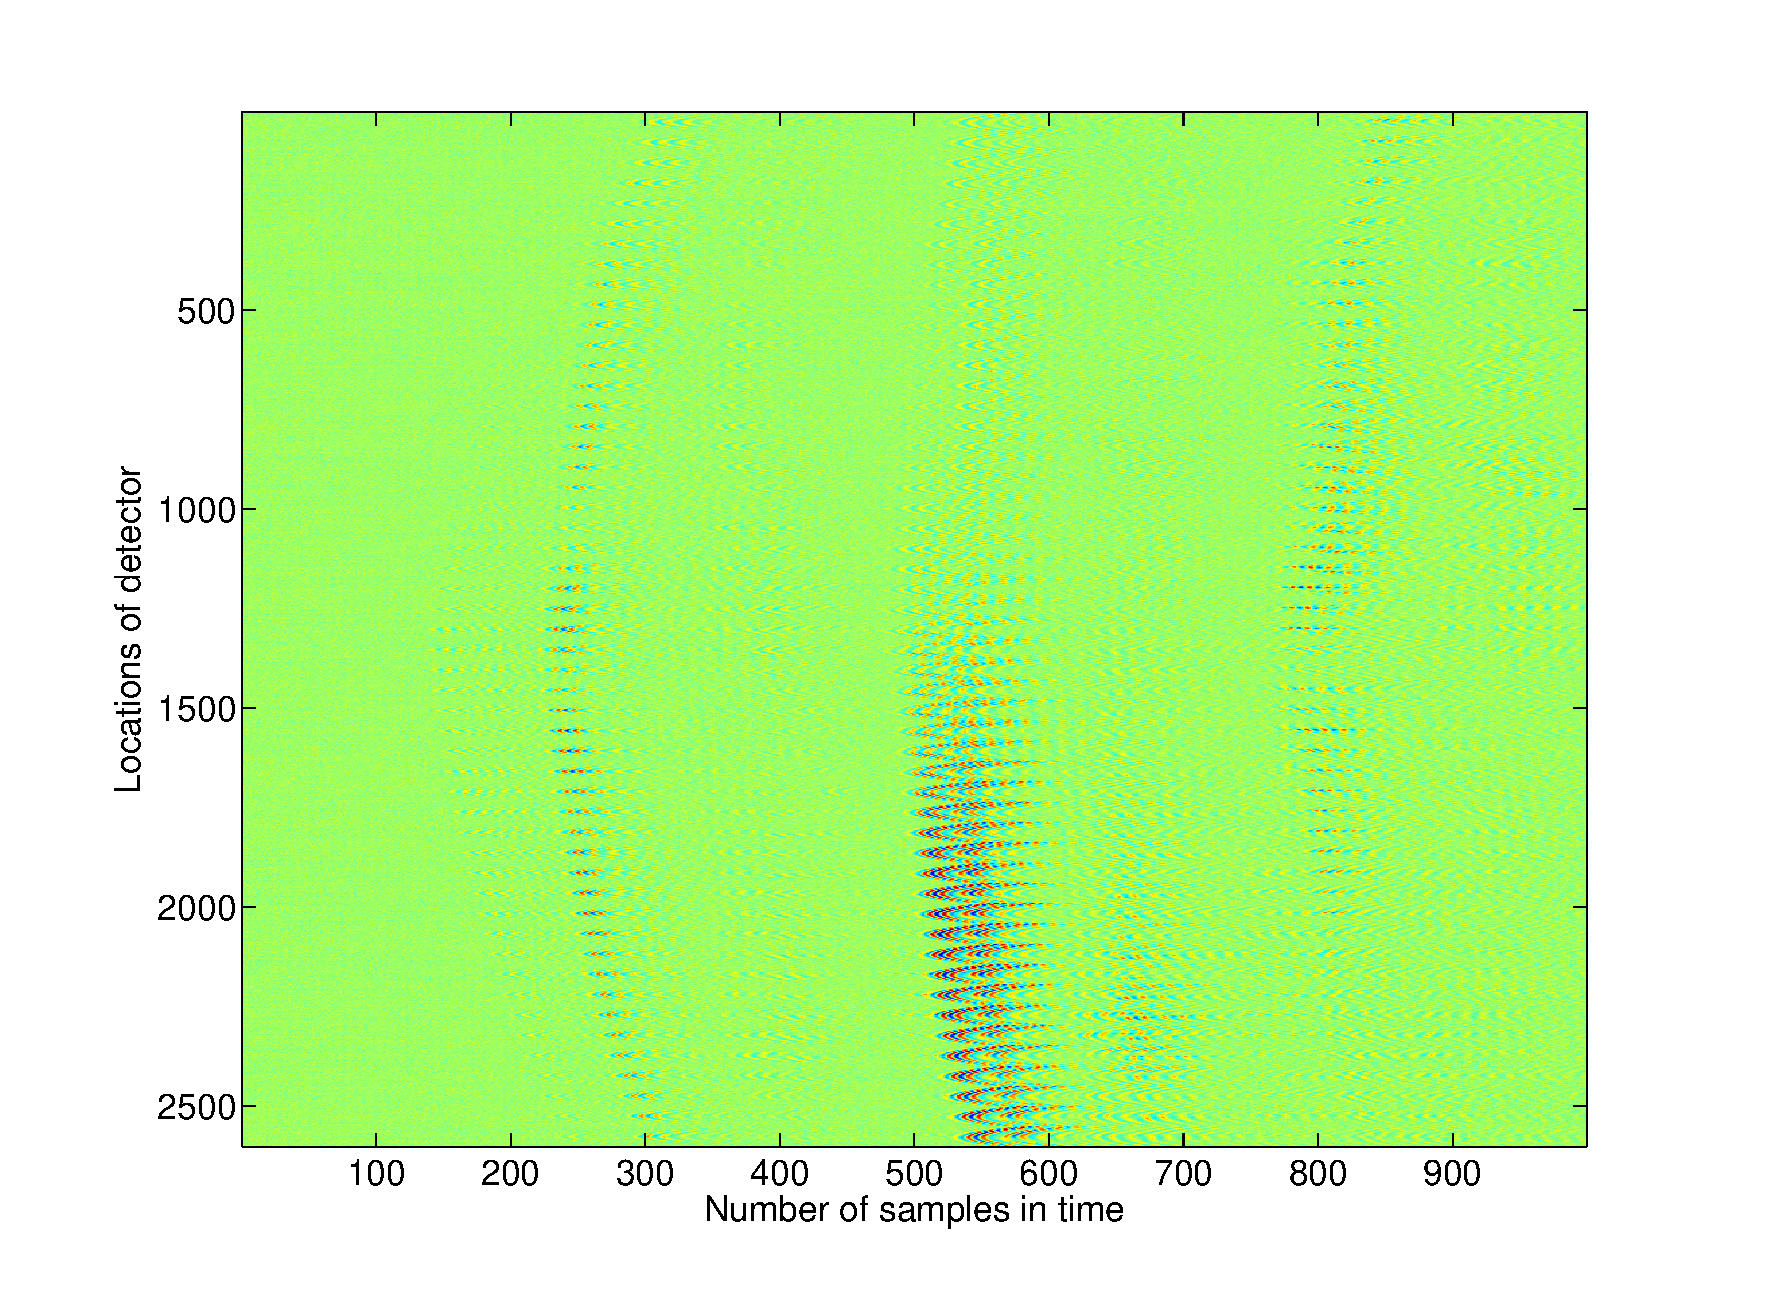
\includegraphics[width=0.48\textwidth]{figure/rawdata_2d}}
 \subfigure[]{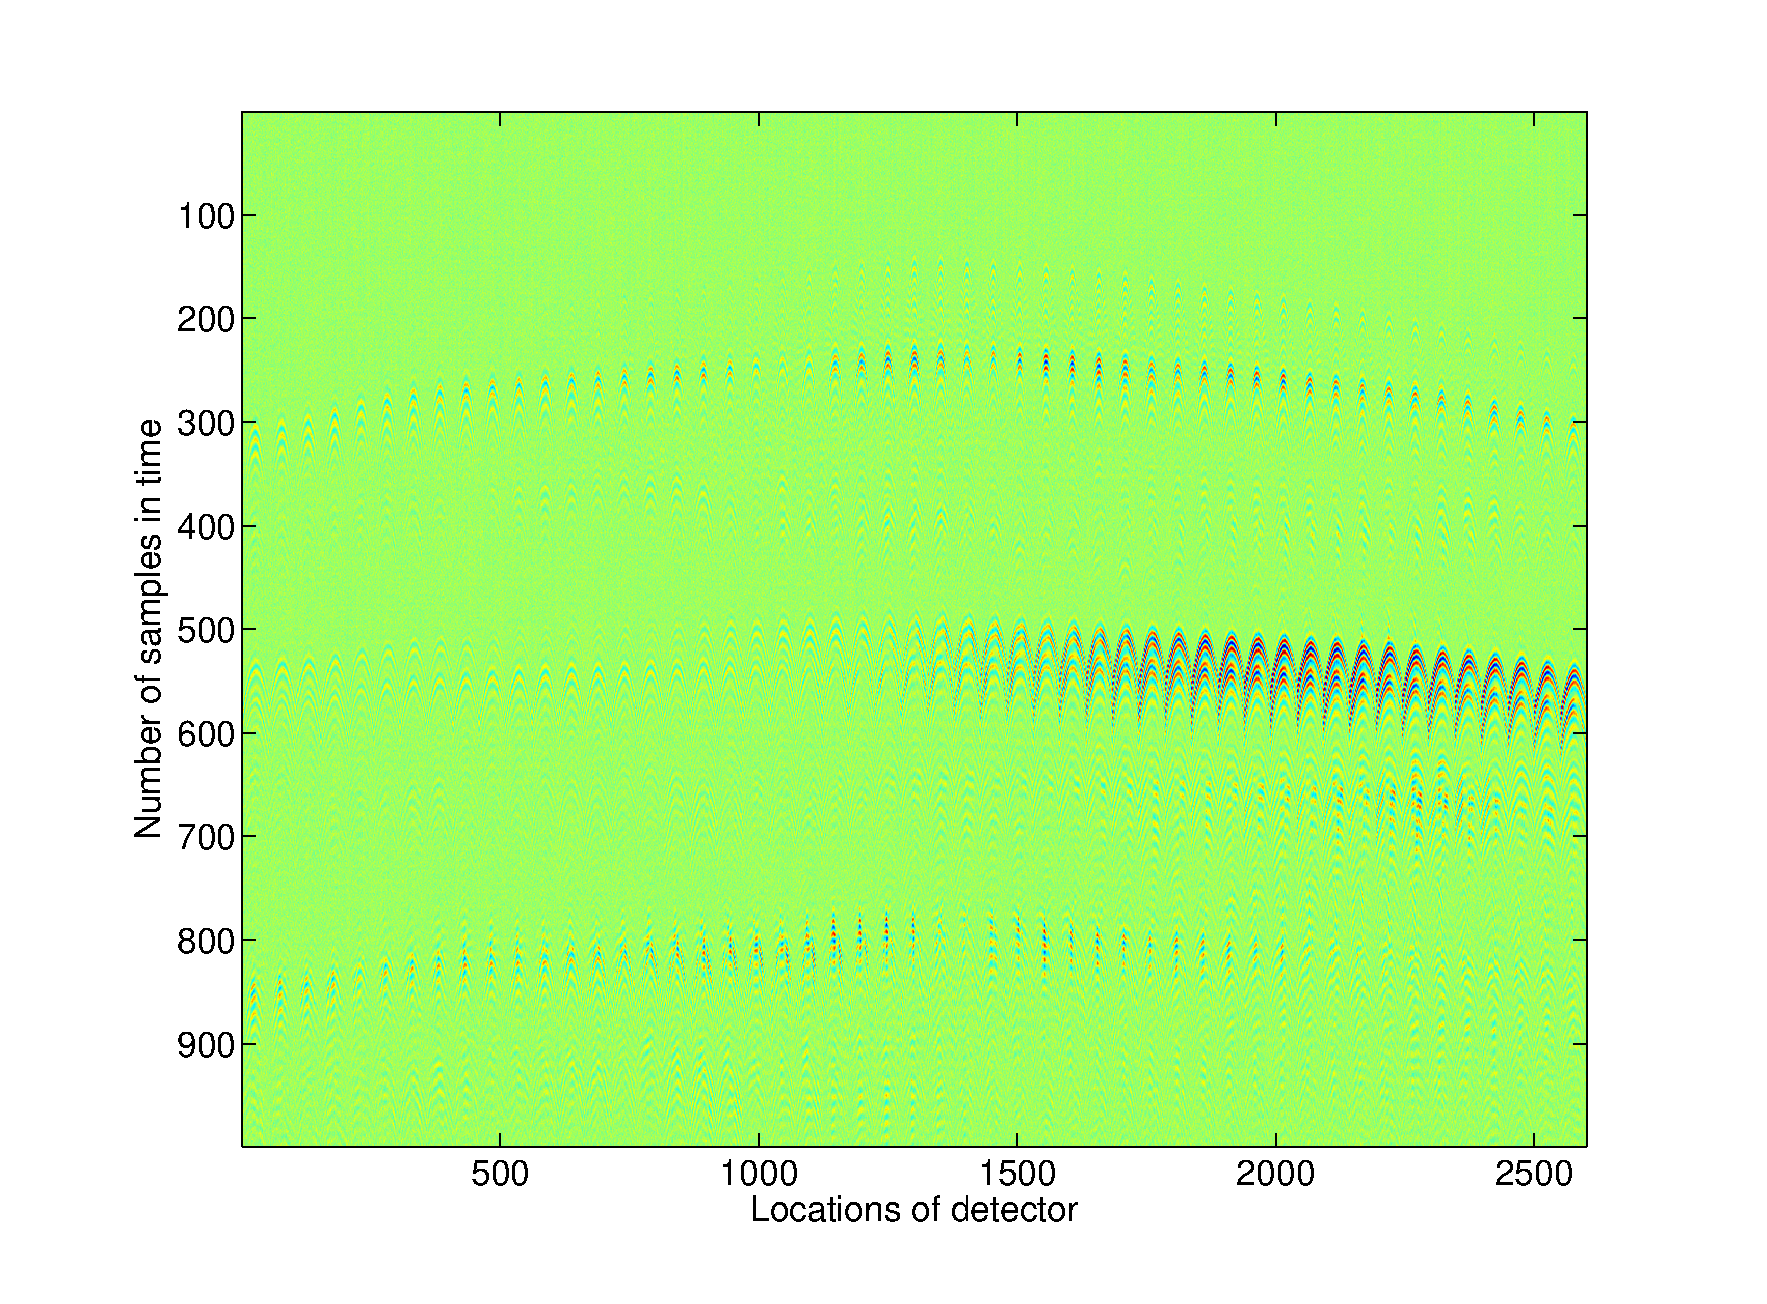
\includegraphics[width=0.48\textwidth]{figure/rawdata_2d_transpose}}
  \caption{(a) A raw data set of a target buried in a sandbox. (b) The transpose of the data in (a). This transposed data is used in data pre-processing.} 
  \label{fig1}
\end{figure}

To pre-process a large number of data sets of each experiment at once in a systematic way, they should be saved in ONE main folder, e.g. ``dataset\_air'' as in ``examples''.  In this main folder, each acquired data set is saved in a list of sub-folders named ``object\_1'', ``object\_2'', ect. Moreover, the measured data MUST have the same file name ``measured\_data.m''. See the folder ``examples'' for examples of data sets. 

The creation of the data folders can be done by calling the MATLAB function ``create\_folders.m'' or just create them manually. 

The incident wave has the form as shown in Figure \ref{fig0}.
\begin{figure}[tph]
   \centering
 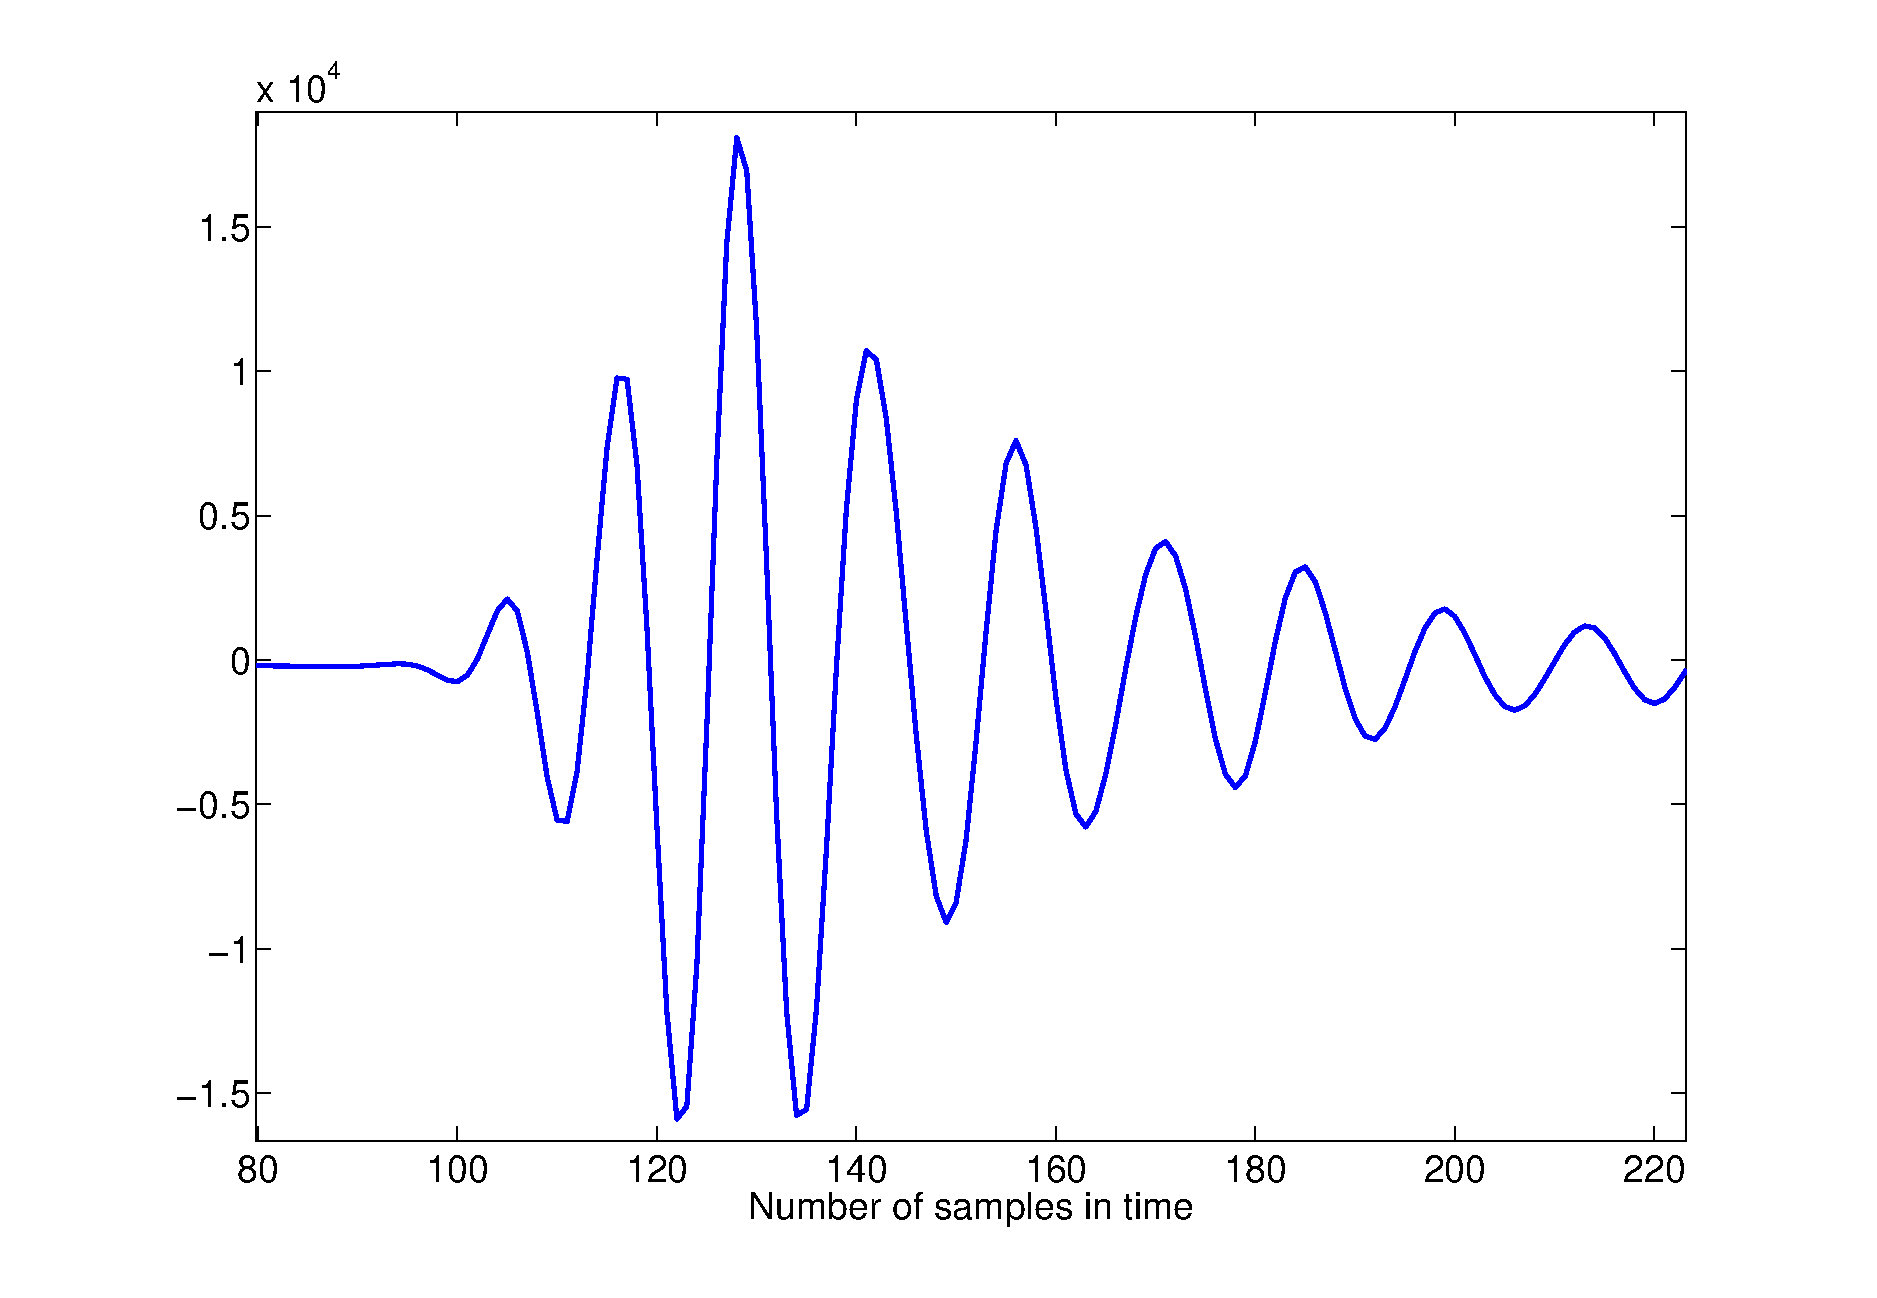
\includegraphics[width=0.6\textwidth]{figure/incident_wave}
  \caption{Waveform of the incident wave.} 
  \label{fig0}
\end{figure}




\subsection{Using the codes}\label{sec:int}

The source codes are in MATLAB. There is another implementation of the codes in C++ but is being updated. This readme file will be updated when the C++ codes are completed. 

\subsubsection{Input parameter file for data pre-processing}
Before running the data pre-processing codes, an input parameter file must be created. You can save to any name you want, but remember to use the same name when you call the pre-processing codes. This file contains the necessary information about the data set, see the file ``parameters\_for\_preprocessing.dat'' in ``examples/data\_sandbox'' to understand its structure and explanations. 

After creating the parameter file, run the Matlab codes as follows. 

\subsubsection{Running the MATLAB codes}

The main function in the MATLAB codes for data pre-processing is \textbf{``data\_preprocessing.m''}. Other functions are called by this one. To call this function, first go to the MAIN folder of the experiment you want to pre-process, e.g. ``dataset\_air'' in ``examples'', as described in the previous section. Then run in the MATLAB command window the following command:

\textit{data\_preprocessing(ObjFolder,ParFile,StartStep,EndStep,HomoSolFile,ScalingFacFile,Shift);}

where 
\begin{itemize}
   \item ObjFolder:  the name of a subfolder which contains one data set. We always create a subfolder for each data set. 
\item ParFile: parameter file for preprocessing, 

see ``examples/dataset\_air/parameters\_for\_preprocessing.dat'' for an example.
\item StartStep: the first step of data preprocessing to be run. This is between 1 and 7. See section \ref{sec:3} for details of each steps. For example, choose this to be 1. 

\item EndStep: the last preprocessing step to be run. Choose this to be 7 as an example. In this case, all steps will be run. 

\item HomoSolFile: this is a file containing the solution of the forward problem in homogeneous medium at the same plane as the propagated data. This file is created by the forward solver WaveES.  

\item ScalingFacFile: this file contains a vector of the scaling factors in Laplace transform, which is the ratio of the experimental data of the calibrating object with that of the simulated data after Laplace transform at a given set of pseudofrequencies. 

See the file ``example/dataset\_air/scaling\_factor\_w\_s9.00\_7.00.m'' for an example.
\item Shift: this is a number which compensate for the shift of the true direct signal from the first detected signal. For UNCC data, this number is 164 if the upsampling factor is chosen to be 2, see the parameter file for the meaning of upsampling factor. 


\end{itemize}

As an example, go to folder ``examples/dataset\_air'' on Matlab, then run the following command: 


\textit{data\_preprocessing('object\_1','parameters\_for\_preprocessing.dat',1 ,4,}

\textit{'hom/Sol\_Z4.m','scaling\_factor\_w\_s9.00\_7.00.m',164);}
 
\subsubsection{Input file for the inverse problem solver}

The input file for the globally convergent method implemented by Larisa of each data set is the file named ``prop\_dat\_inv\_scale\_v\_....m''. 

The input file for Thanh's implementation of the globally convergent method of each data set is the file named ``boundarydata\_s...m''. 

\subsection{Steps of data pre-processing}\label{sec:3}

In this section, a data set is represented by a matrix $G = \{G_{mn}\}$ whose columns are time-dependent data at the locations of the detector. 

\subsubsection{Off-set correction}

This step is to shift the recorded data to zero-offset, that means, the mean value (or the zero frequency data) of each time-dependent curve should be zero. Denote by $G_{n}$ the $n$th column of the measured data. The zero-offset is corrected using the following formula:
$$
G^{corrected}_{n} = G_{n} - \text{mean}  (G_{n}).
$$

\subsubsection{Upsampling}
Upsampling means increasing the sampling rate (or decreasing the time step) by interpolating the data in time. This step is needed in case if the forward solver needs a small time step to make the numerical solution stable. In the current code, we use the linear interpolation or zero-padding. 


\subsubsection{Time zero correction}

Time-zero refers to the moment at which the signal is emitted from the transmitter. The recorded
signals may be shifted in time. Without time-zero correction, we are not be able to estimate the distance from the antennas to the objects. Therefore this step is needed in data preprocessing. 

We use the direct signal (the signal which travels directly from the transmitter to the detector without interference with other objects) for this purpose. This should be the first signal seen in the data. The time-zero correction is done as follows:

\begin{figure}[tph]
   \centering
 \subfigure[]{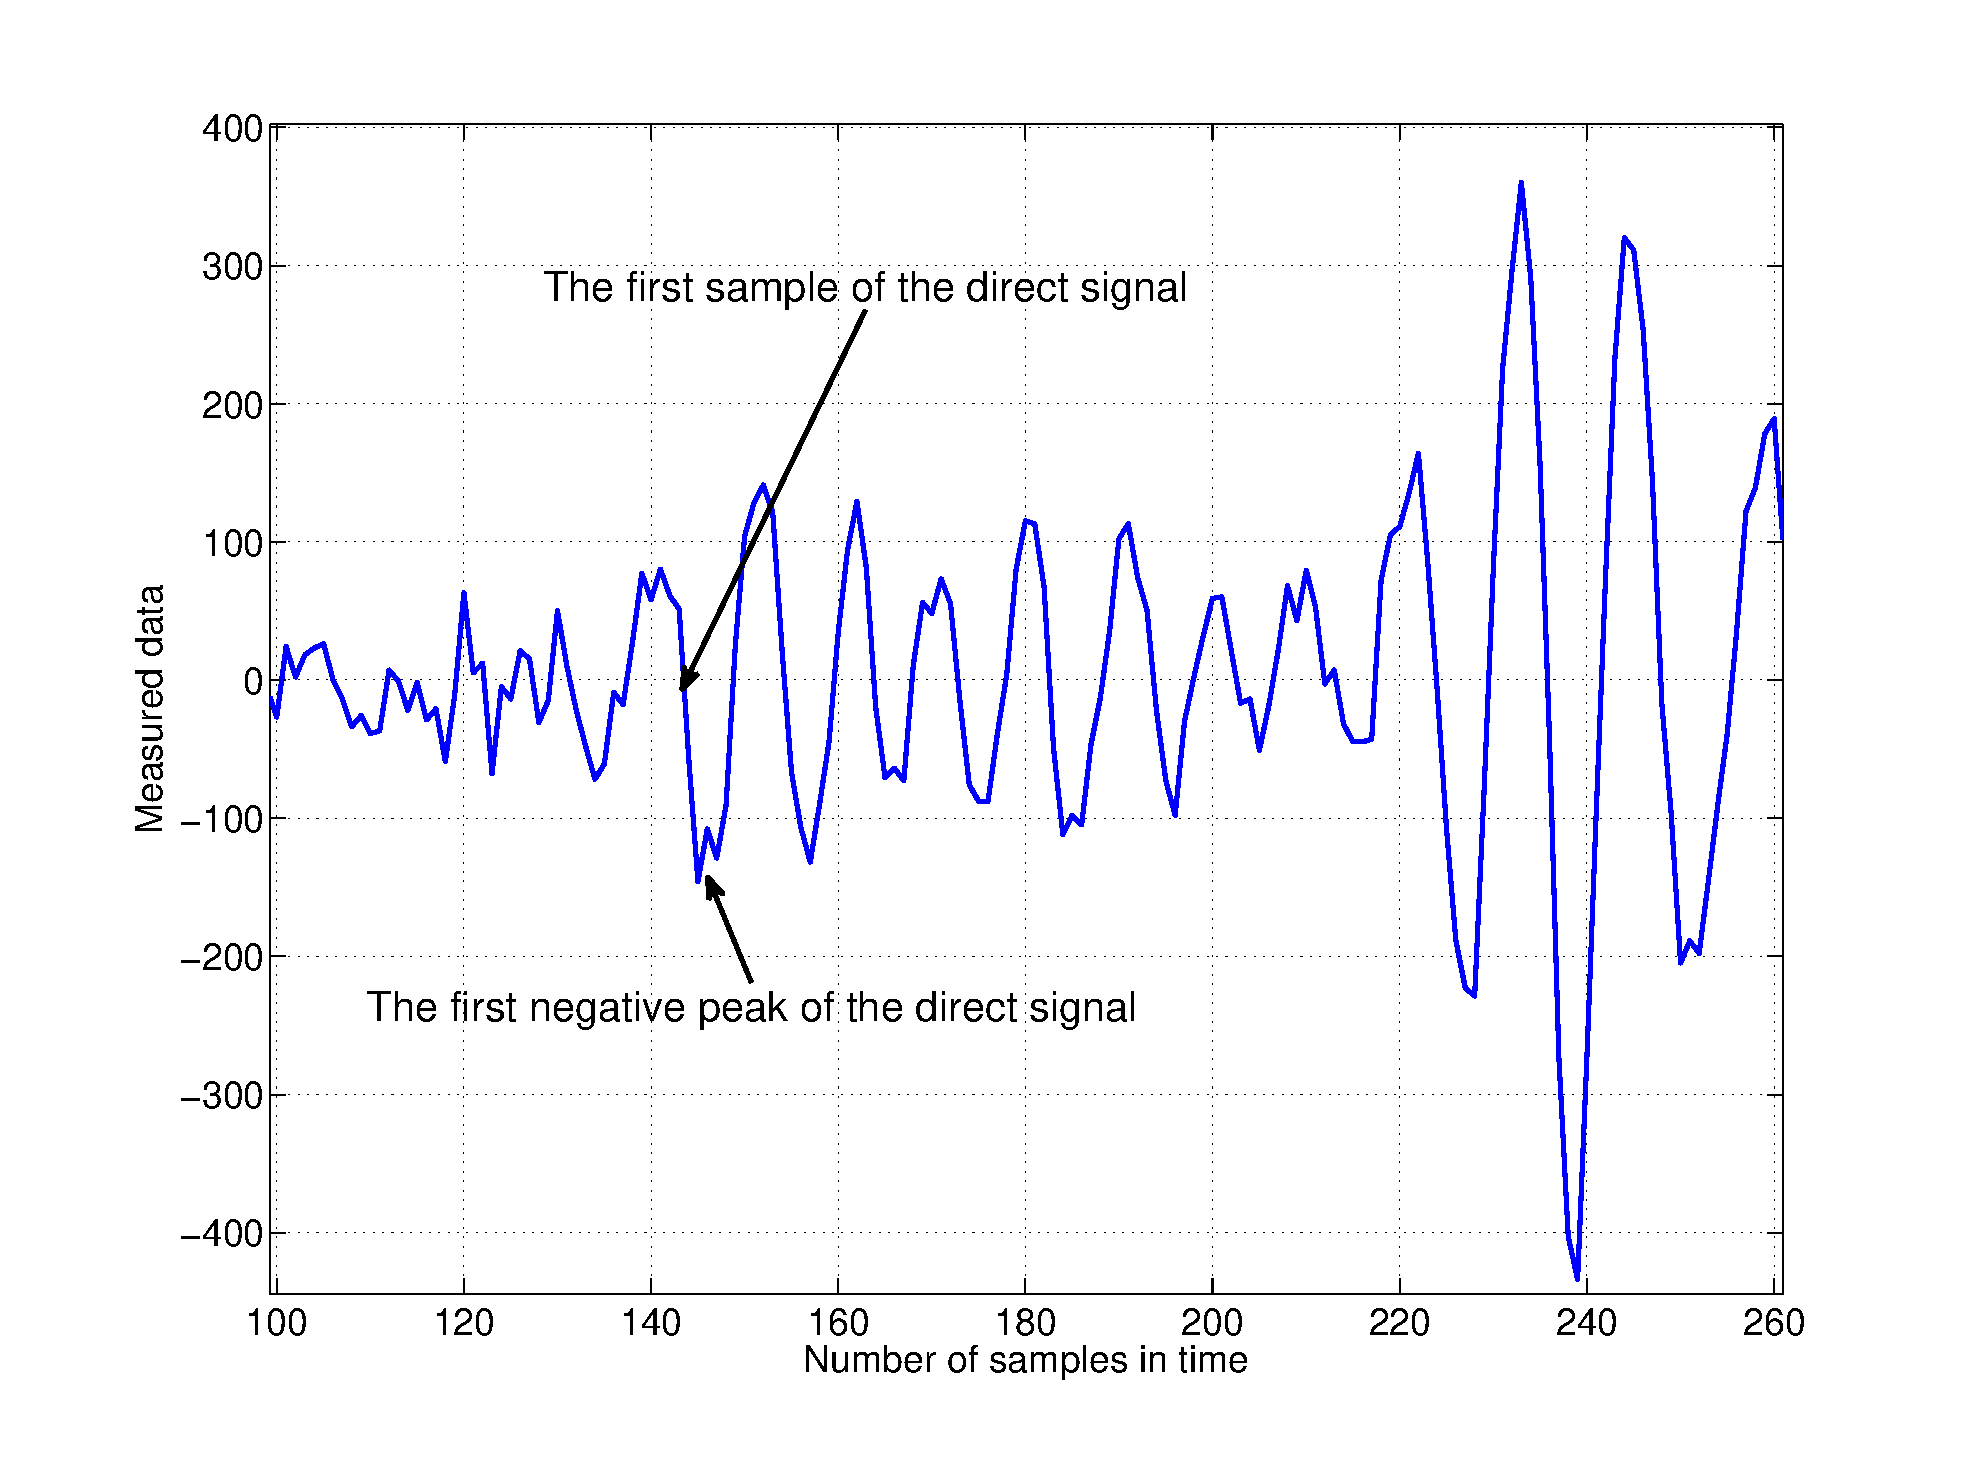
\includegraphics[width=0.65\textwidth]{figure/timezero_1}}

 \subfigure[]{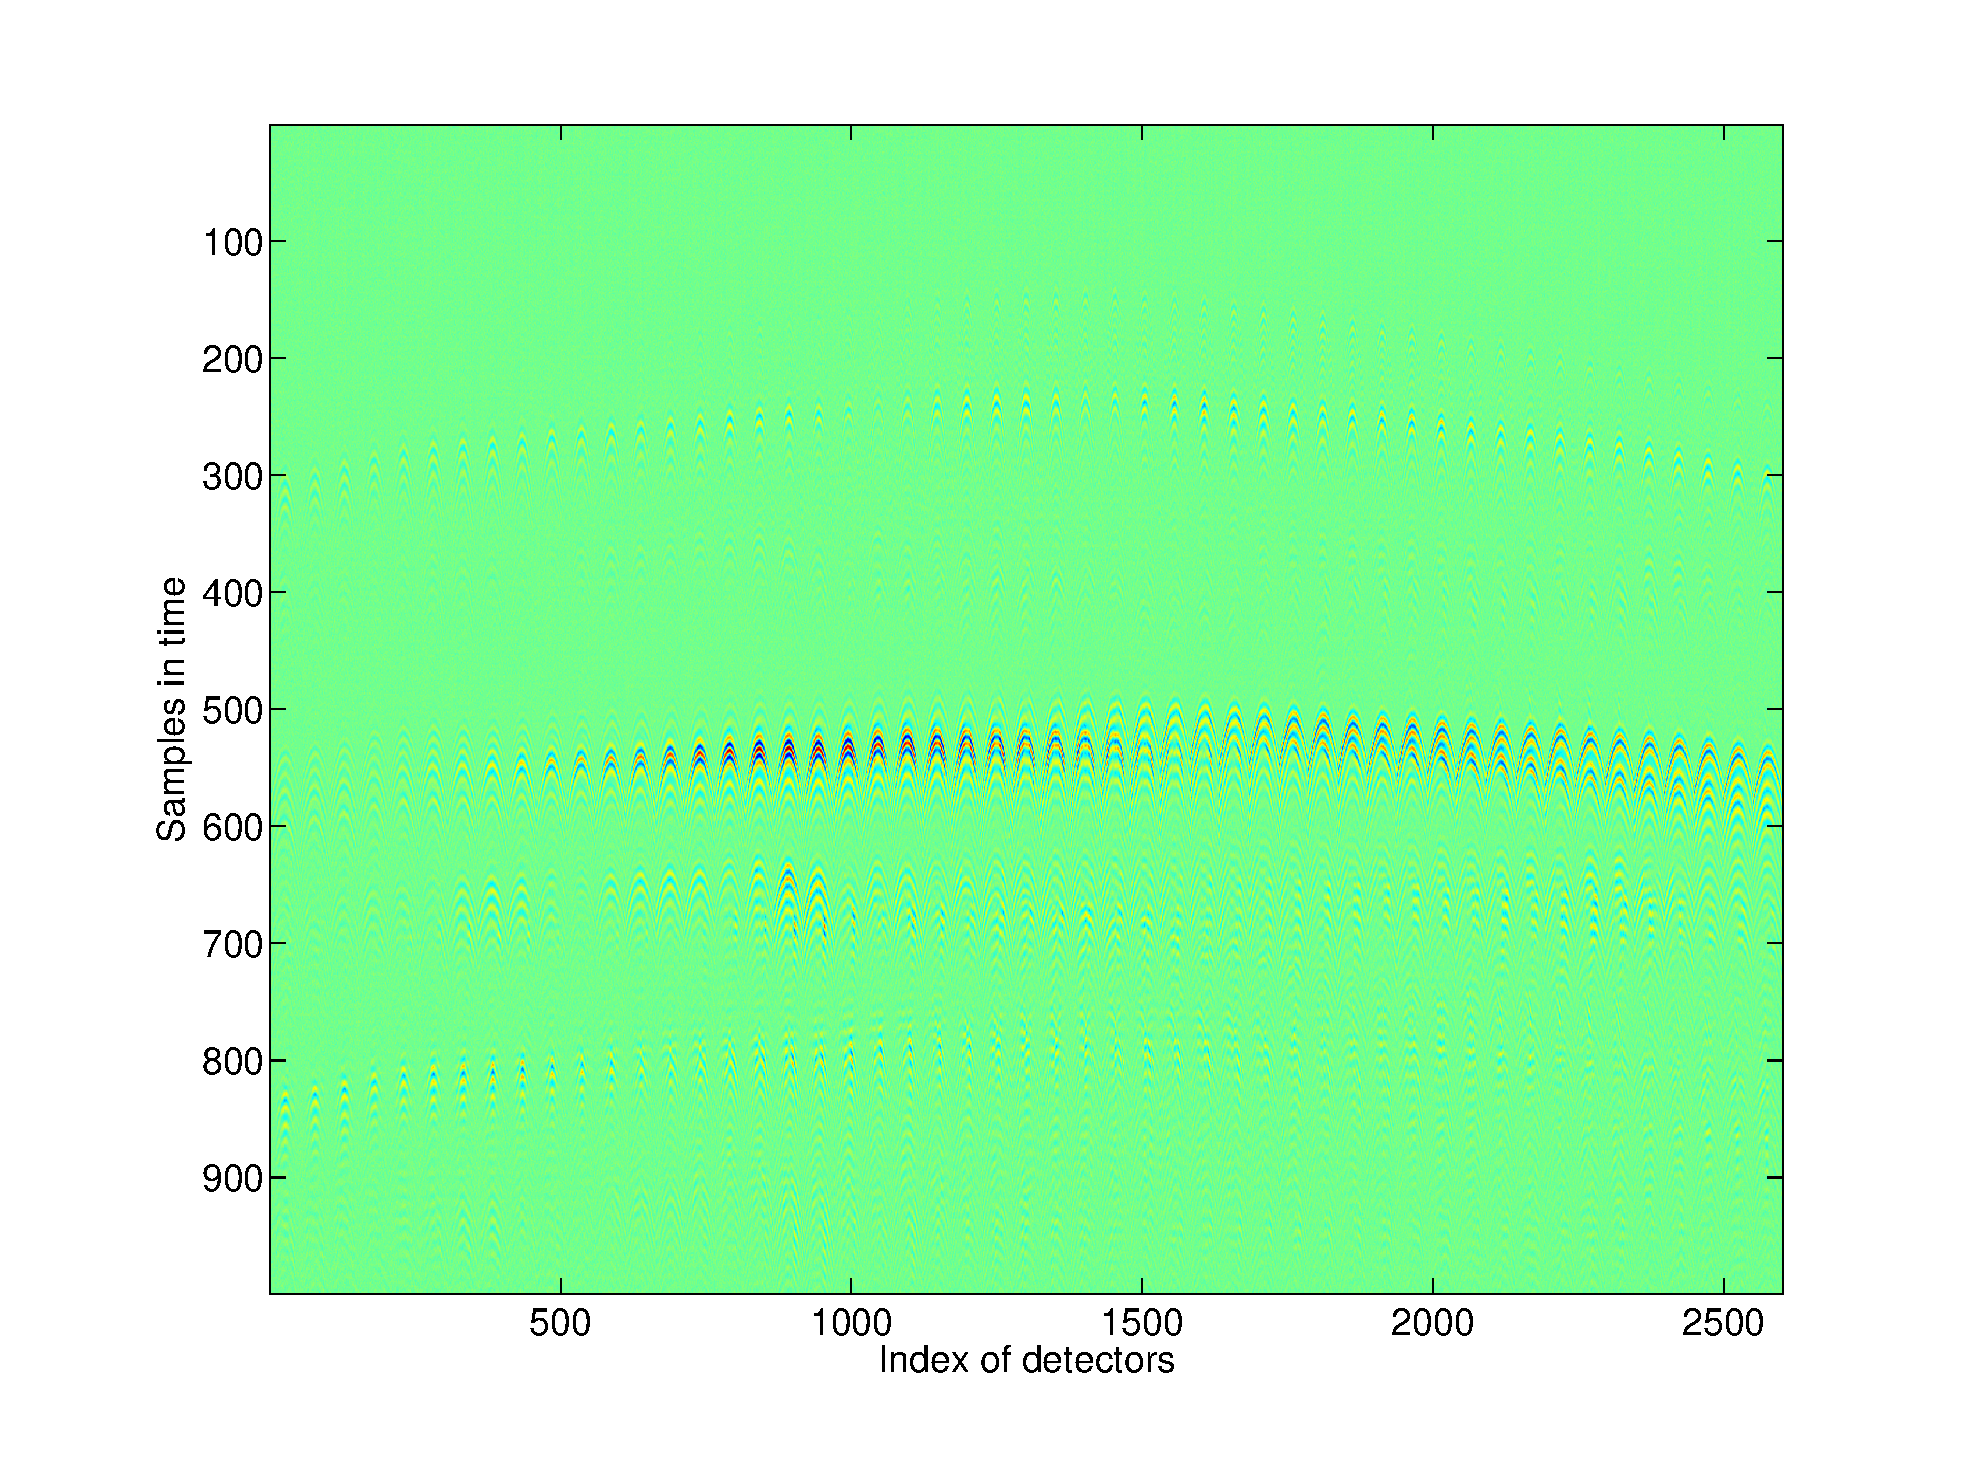
\includegraphics[width=0.49\textwidth]{figure/timezero_2}}
 \subfigure[]{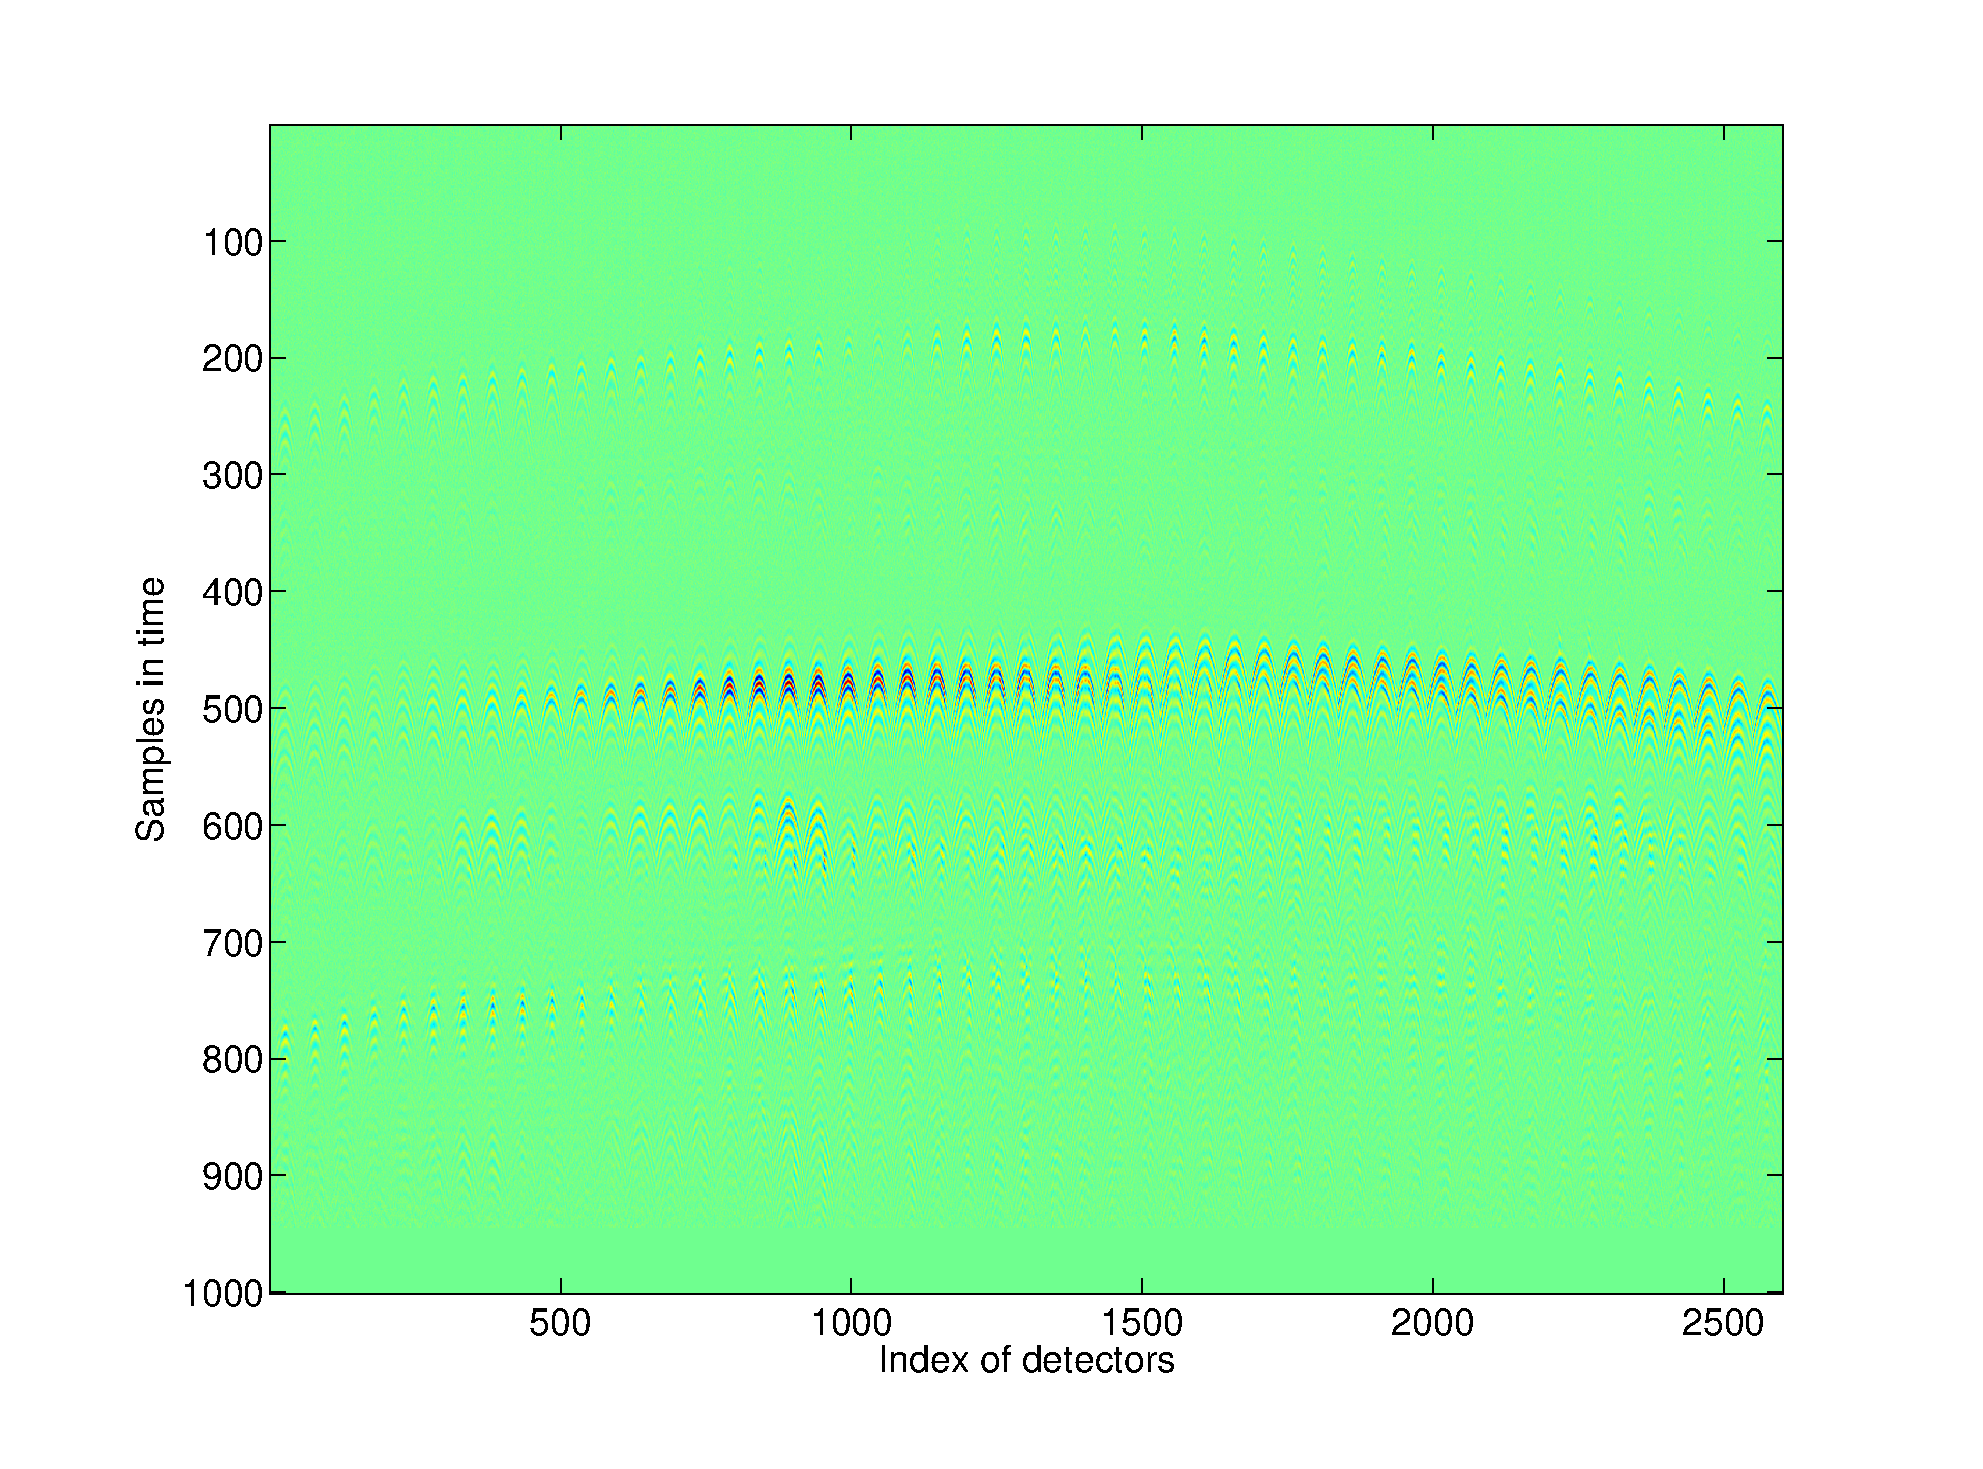
\includegraphics[width=0.49\textwidth]{figure/timezero_3}}
  \caption{Time zero correction: (a) the first negative peak and the first sample of the direct signal. (b) The 2-d data before time zero correction. The 2-d data after time zero correction. Notice the time shift between b) and c).} 
  \label{fig2}
\end{figure}


\begin{enumerate}
   \item First, we choose the detector at the center of the measurement plane as the time-dependent data at this detector has the strongest direct signal. In our data, this is the detector number $1301$. 
   \item Second, we detect the first peak of the direct signal, see Figure \ref{fig2}. We can choose this peak as the first negative peak which is stronger than a given noise level in amplitude. The noise level MUST be provided (by the user) for each radar device. 
  \item Third, we choose the last positive sample before the detected peak. We can choose this or the next sample as the first sample of the direct signal. Note that we do not choose the first peak as the first sample of the direct signal. 
  \item Fourth, we calculate the time delay and the corresponding number of samples for the wave to travel from the transmitter to the detector, GIVEN the correct distance from them and the recorded (after upsampling, if applied) time step. 
  \item Shift the data in time according to the estimated number of samples. 
\end{enumerate}

\subsubsection{Data propagation}
In this step, the data is propagated to a plane, which we refer to as the \textit{propagated plane}.
This plane is located closer to the targets than the measurement plane. This
means that we approximate the scattered wave on the propagated plane using
the measured scattered wave on the measurement plane. There are two reasons
for doing this. The first one is that since the kernel
of the Laplace transform decays exponentially with respect to
time, which is proportional to the distance from the targets to the
measurement plane, then the amplitude of the data after the Laplace
transform on the measurement plane is very small and can be dominated by the
computational error. The second reason is that the data propagation
procedure helps to reduce the computational cost substantially since the
size of the computational domain is reduced. We have also observed
that the data propagation helps to reduce the noise in the measured data and focus the signal around the location of the targets. See the papers \cite{TBKF:SISC2014,TBKF:2013-2} for details of two data propagation methods: time-reversal and Fourier transform methods.




\begin{figure}[tph]
\centering
\subfigure[Before propagation]{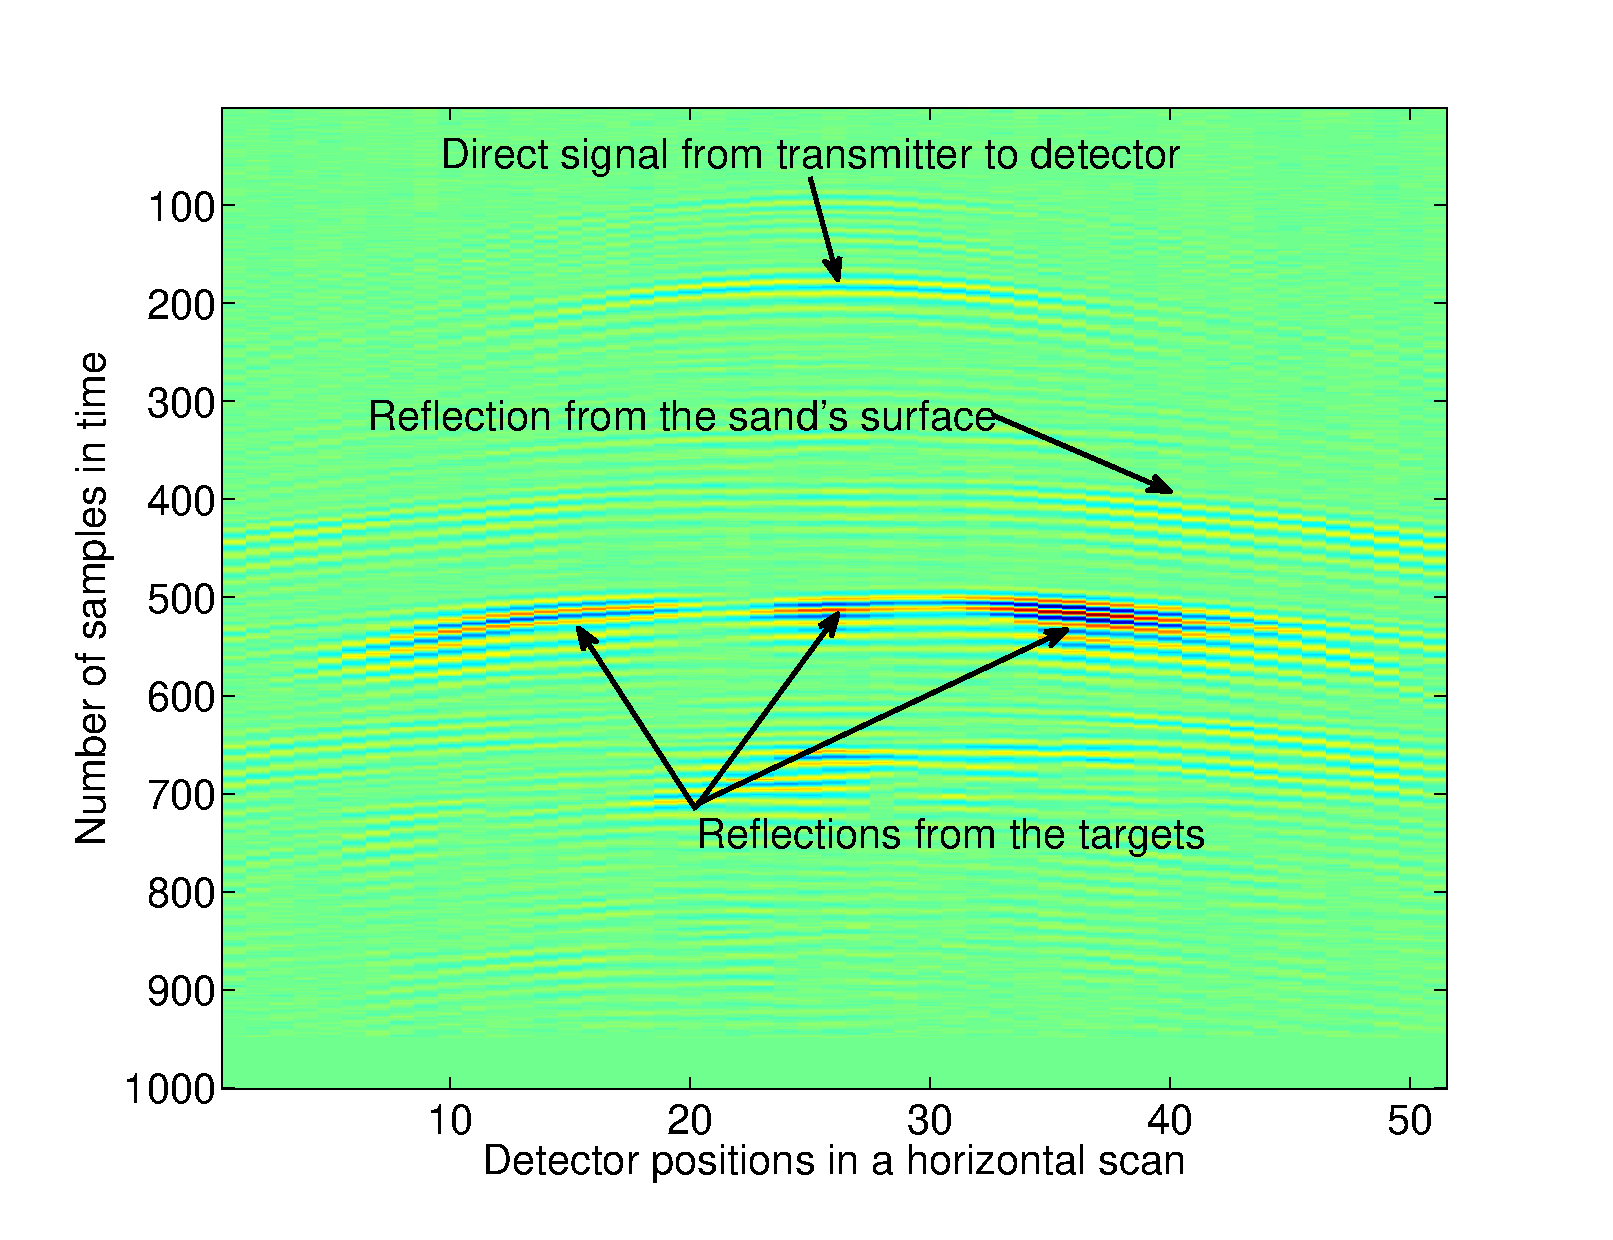
\includegraphics[width =
0.48\textwidth]{figure/Figure9_a2}} 
\subfigure[After
propagation]{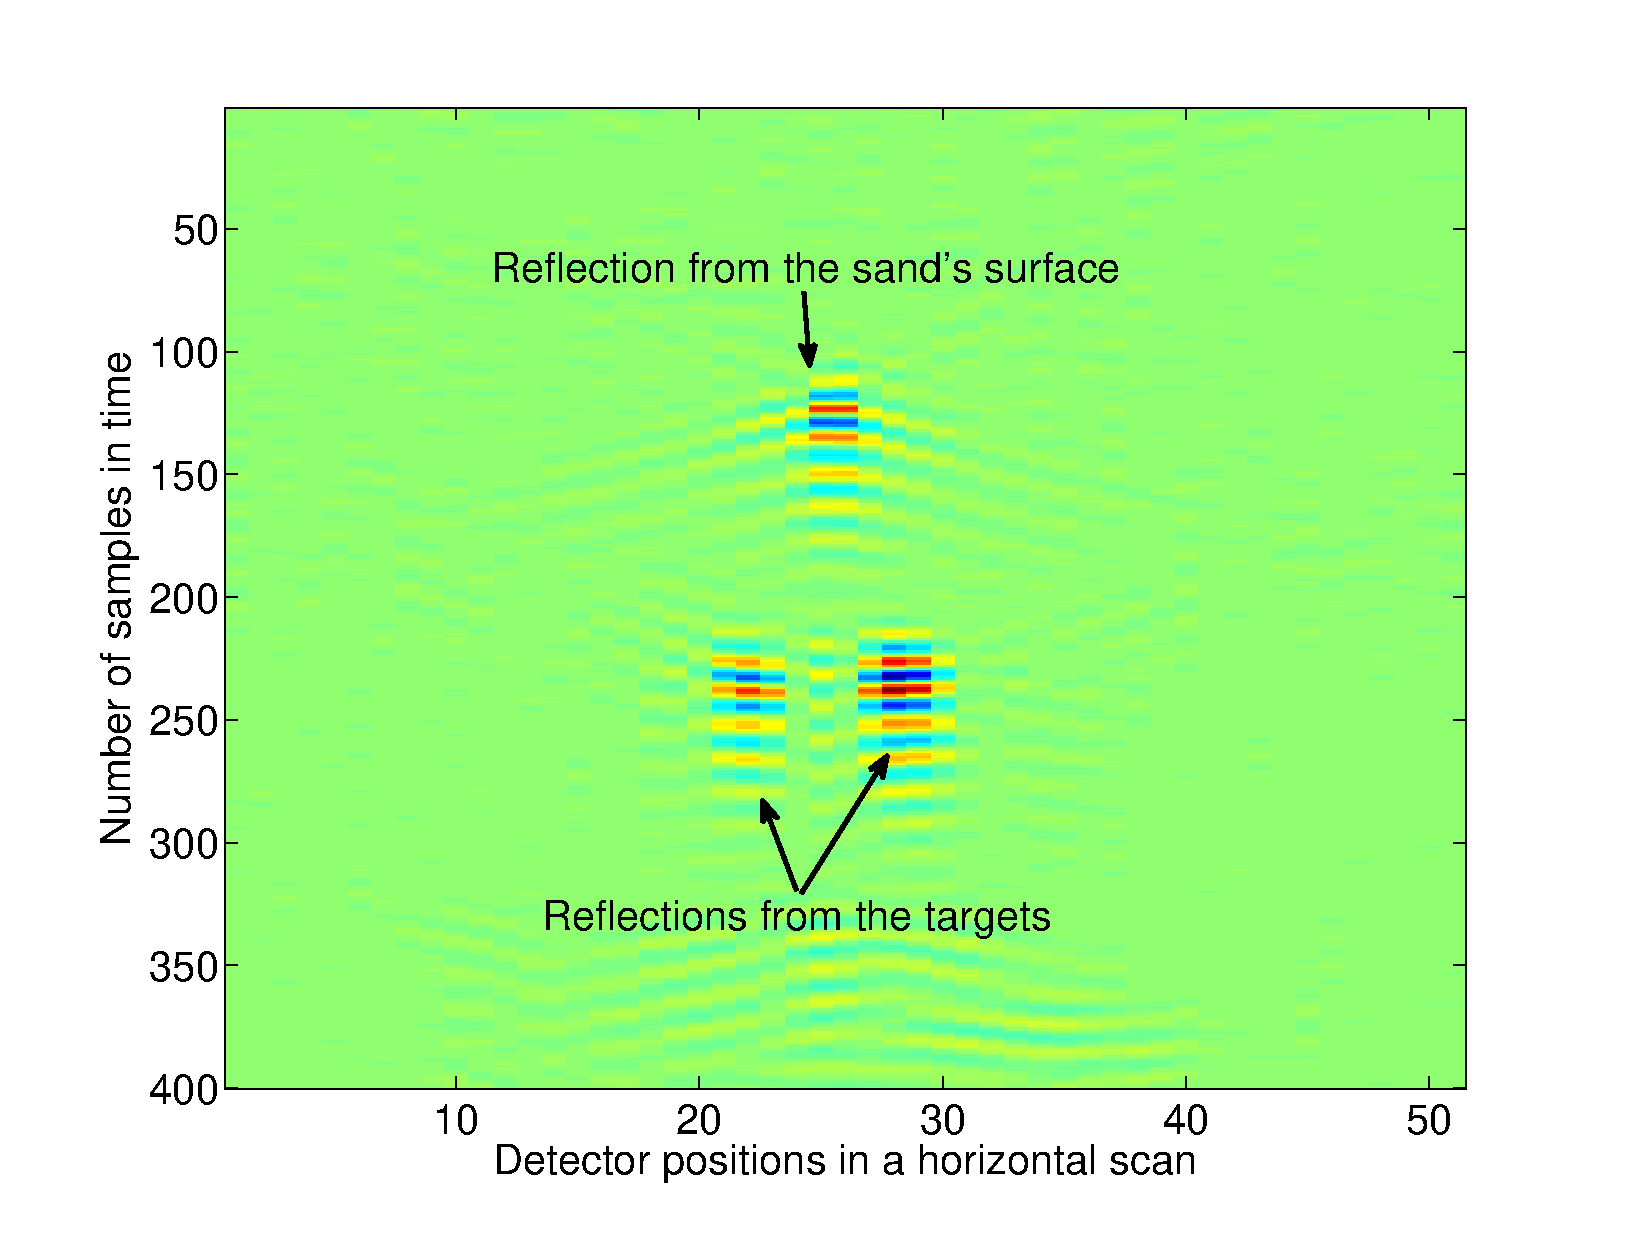
\includegraphics[width = 0.48\textwidth]{figure/Figure9_b2}}
\caption{Result of the data propagation for signals from two targets buried
inside a sand box. The signals of the two targets are well separated from
each other as well as from the reflection from the sand's surface after the
data propagation.}
\label{fig:dataprop}
\end{figure}

A result of the data propagation is illustrated in Figure \ref{fig:dataprop}. The figure shows a horizontal scan of a sand box containing two buried
metallic targets. The horizontal side denotes the indices of the detector's
locations and the vertical side denotes time. Time increases from the top to
the bottom. The propagation distance, $b-a$, is $0.8$ m, which means that
the data after the propagation is approximately at the sand's surface.
Figure \ref{fig:dataprop}(a) shows the original data while Figure \ref%
{fig:dataprop}(b) shows the data after the propagation. As can be seen from
these figures, the targets' signals in the original data are smeared out. On
the other hand, they are focused after the data propagation making the two
targets more clearly distinguished. This is well known for migration
methods. Moreover, we can also see that the reflection from the sand's
surface is also more visible after the propagation and is well separated
from the targets' signals.


The distance from the measurement plane to the propagated plane can be given by the user or estimated. The default propagation distance is taken from the estimated one. 


\subsubsection{Source shift}

In our simulation, we assume that the incident plane wave is emitted on the $\{z = z_0\}$. Therefore, the computational cost depends on the distance from this plane to our targets. To avoid unnecessary
computational cost in our forward and inverse solvers, we artificially shift
the source closer to the sand box. This is done by shifting the whole
time-dependent data by a number of samples which correspond to the time delay between old and new transmitter's locations. 



\begin{figure}[tph]
\centering
\subfigure[]{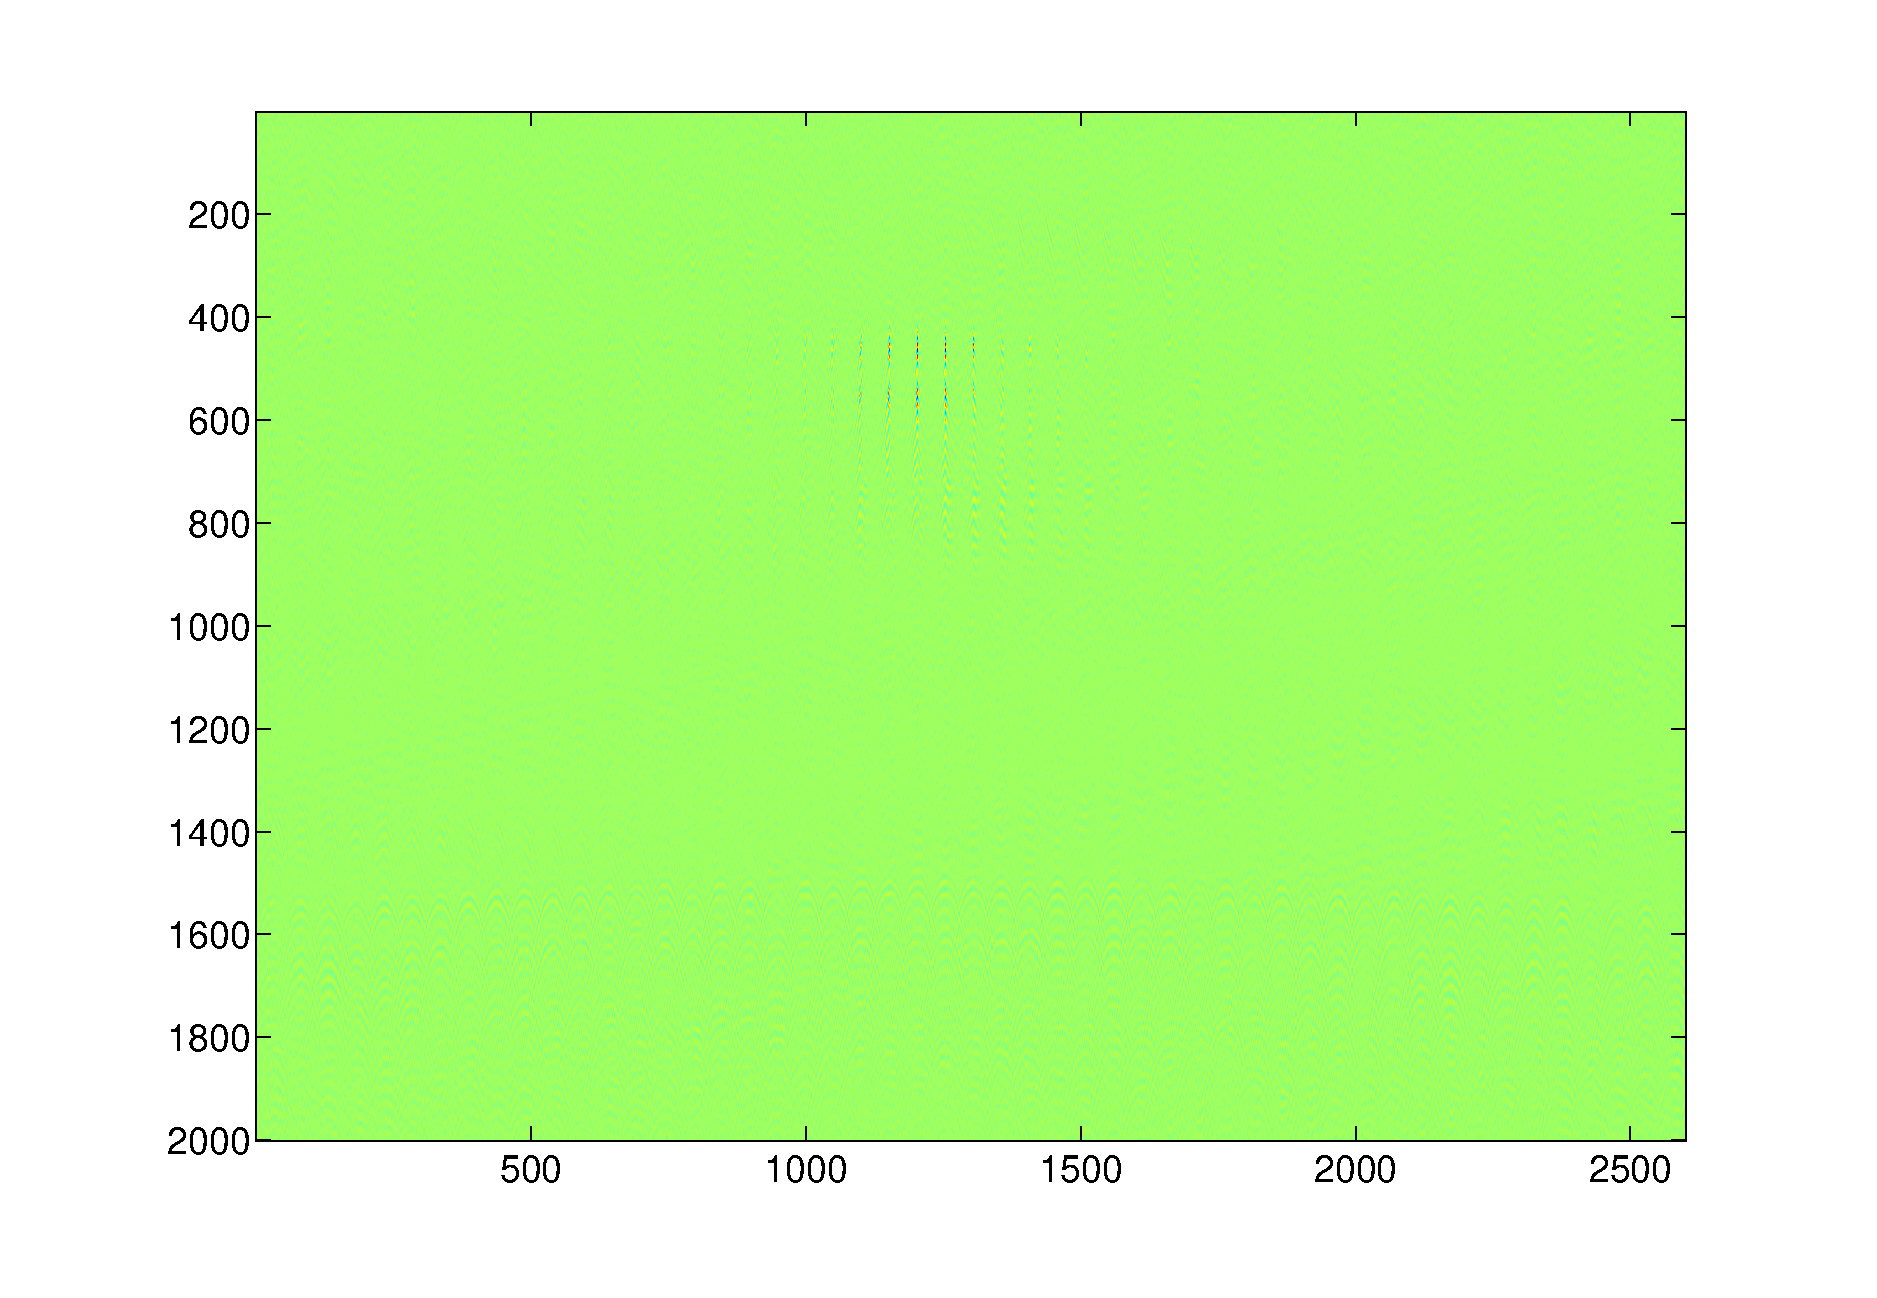
\includegraphics[width = 0.48\textwidth]{figure/prop_dat}} 
\subfigure[]{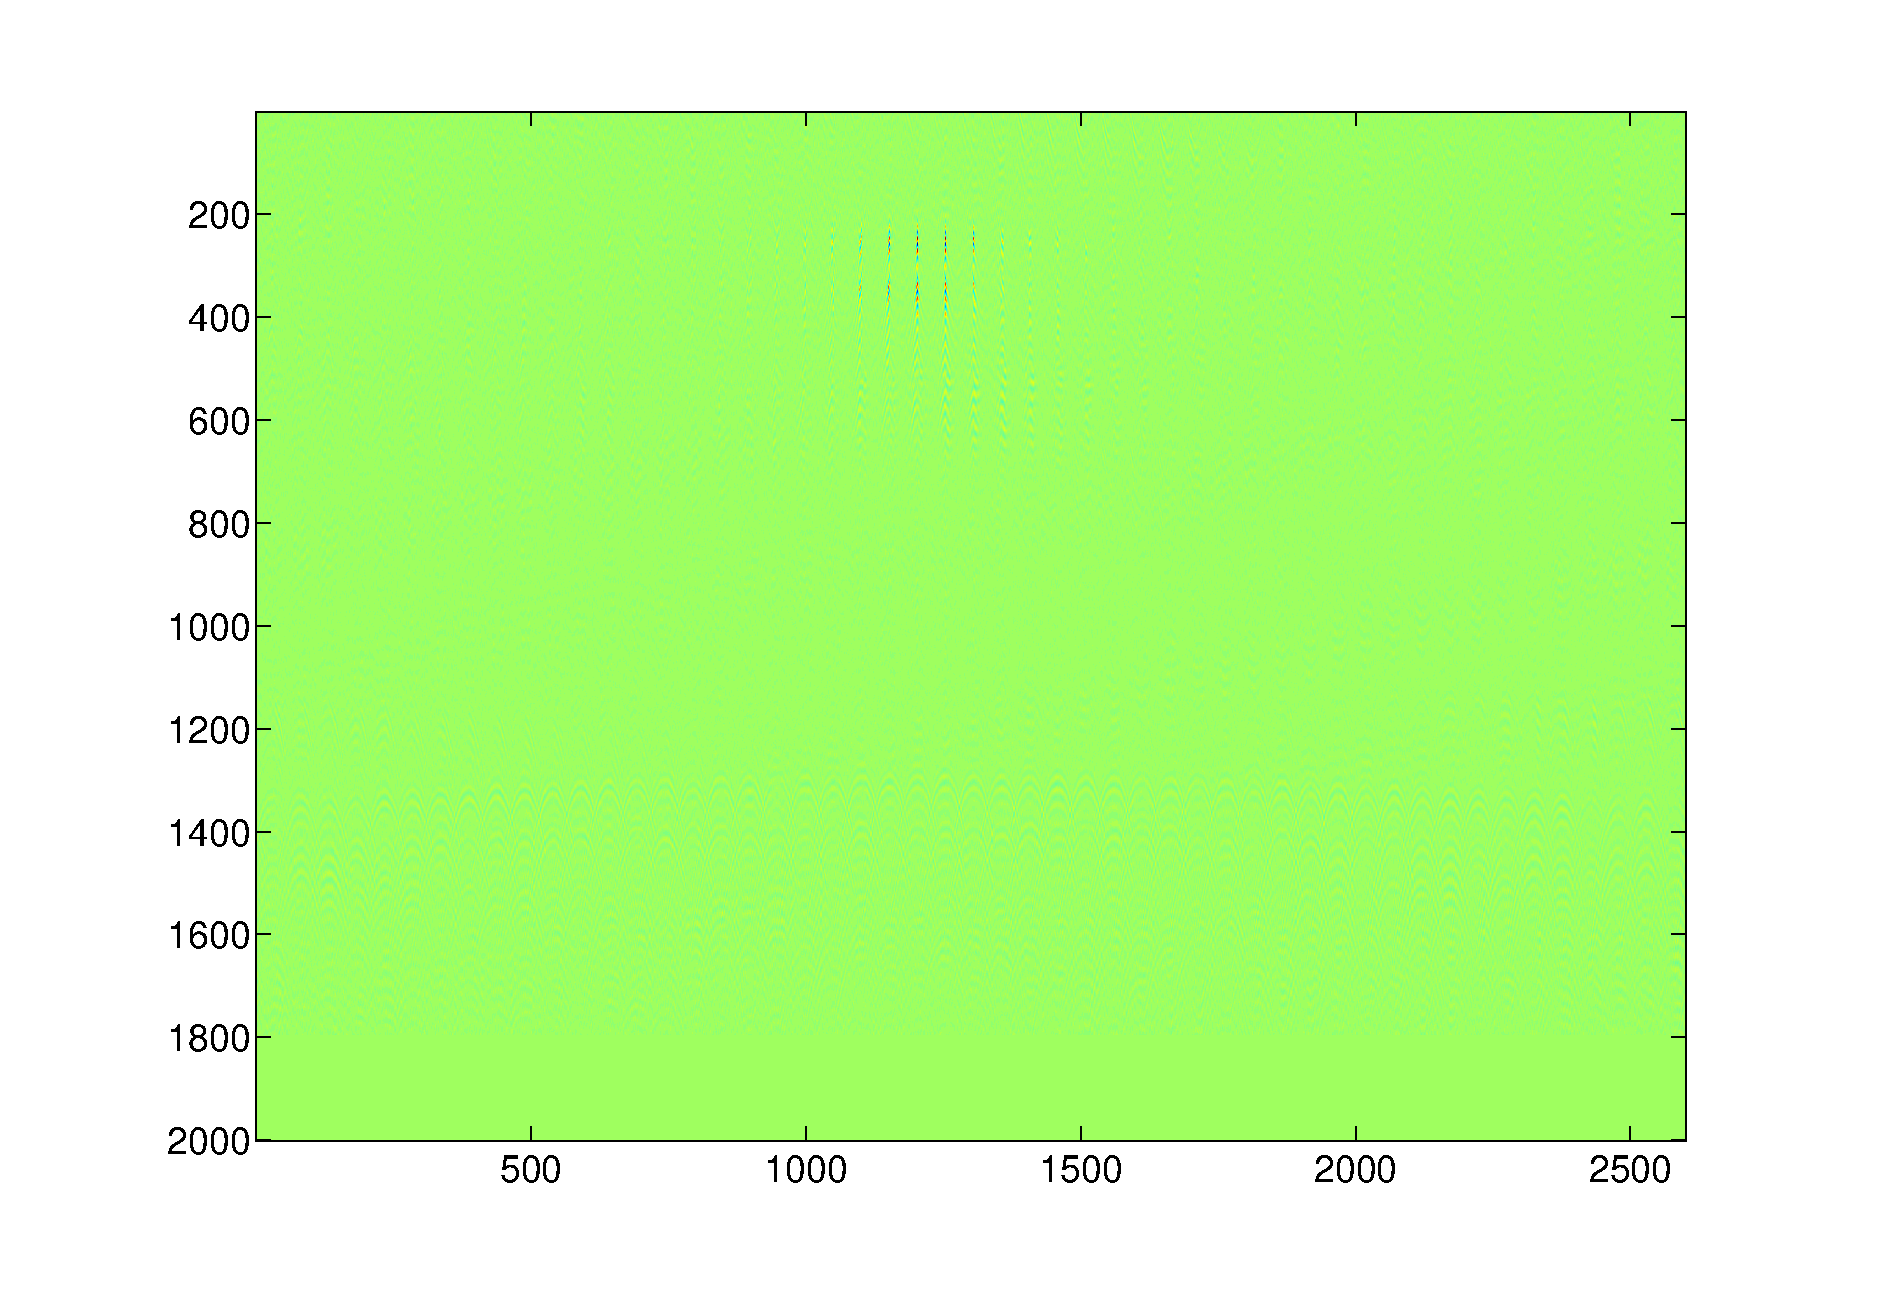
\includegraphics[width = 0.48\textwidth]{figure/source_shift}}
\caption{(a) Propagated data before the source shift, (b) after source shift.}
\label{fig:shift}
\end{figure}

\subsubsection{Estimation of depth and extraction of target's signal}
Apart from the
signals scattered from the targets, our measured data also contain various
types of unwanted signals and noise. The unwanted signals which come
earlier than the targets' signals dominate the latter after the Laplace
transform. Thus, this step helps to remove both these unwanted signals and noise. 


The papers \cite{TBKF:SISC2014} and \cite{TBKF:2013-2} describe in detail about how the target's signal is determined and extracted for the case of targets in air and buried in a sand box, respectively. In particular, the depth of burial is determined as follows:


\begin{enumerate}
   \item Choose the strongest detector, see the definition in \cite{TBKF:2013-2}. 
    \item Determine the largest negative peaks of the sand and the target. The largest negative peak of the target is determined as the one that follows the first four peaks of the data, which should belong to the sand's signal. 
    \item From the time delay between these two peaks, we determine the depth of burial, see section 4.2.2 in \cite{TBKF:2013-2}. 
    \item If the estimated depth is less than 5 cm and if the target's peak is stronger than that of the sand, we conclude that it is a strong target and choose as the starting peak of the target the largest negative one after removing the sand's signal. 
    \item If the estimated depth is less than 5 cm but the target's peak is weaker than that of the sand, we consider it as a weak target and choose as the starting peak of the target the largest positive peak after removing the sand's signal.
    \item If the estimated depth is more than 5 cm, we consider the target as a strong one. In this case, the first peak of the target is chosen to be the largest negative one after removing the sand's signal. 
\end{enumerate}

See Figure \ref{fig:4.30} for an example how to choose the largest negative peaks of the sand and the target as well as the time delay between them. 

\begin{figure}[tph]
\centering
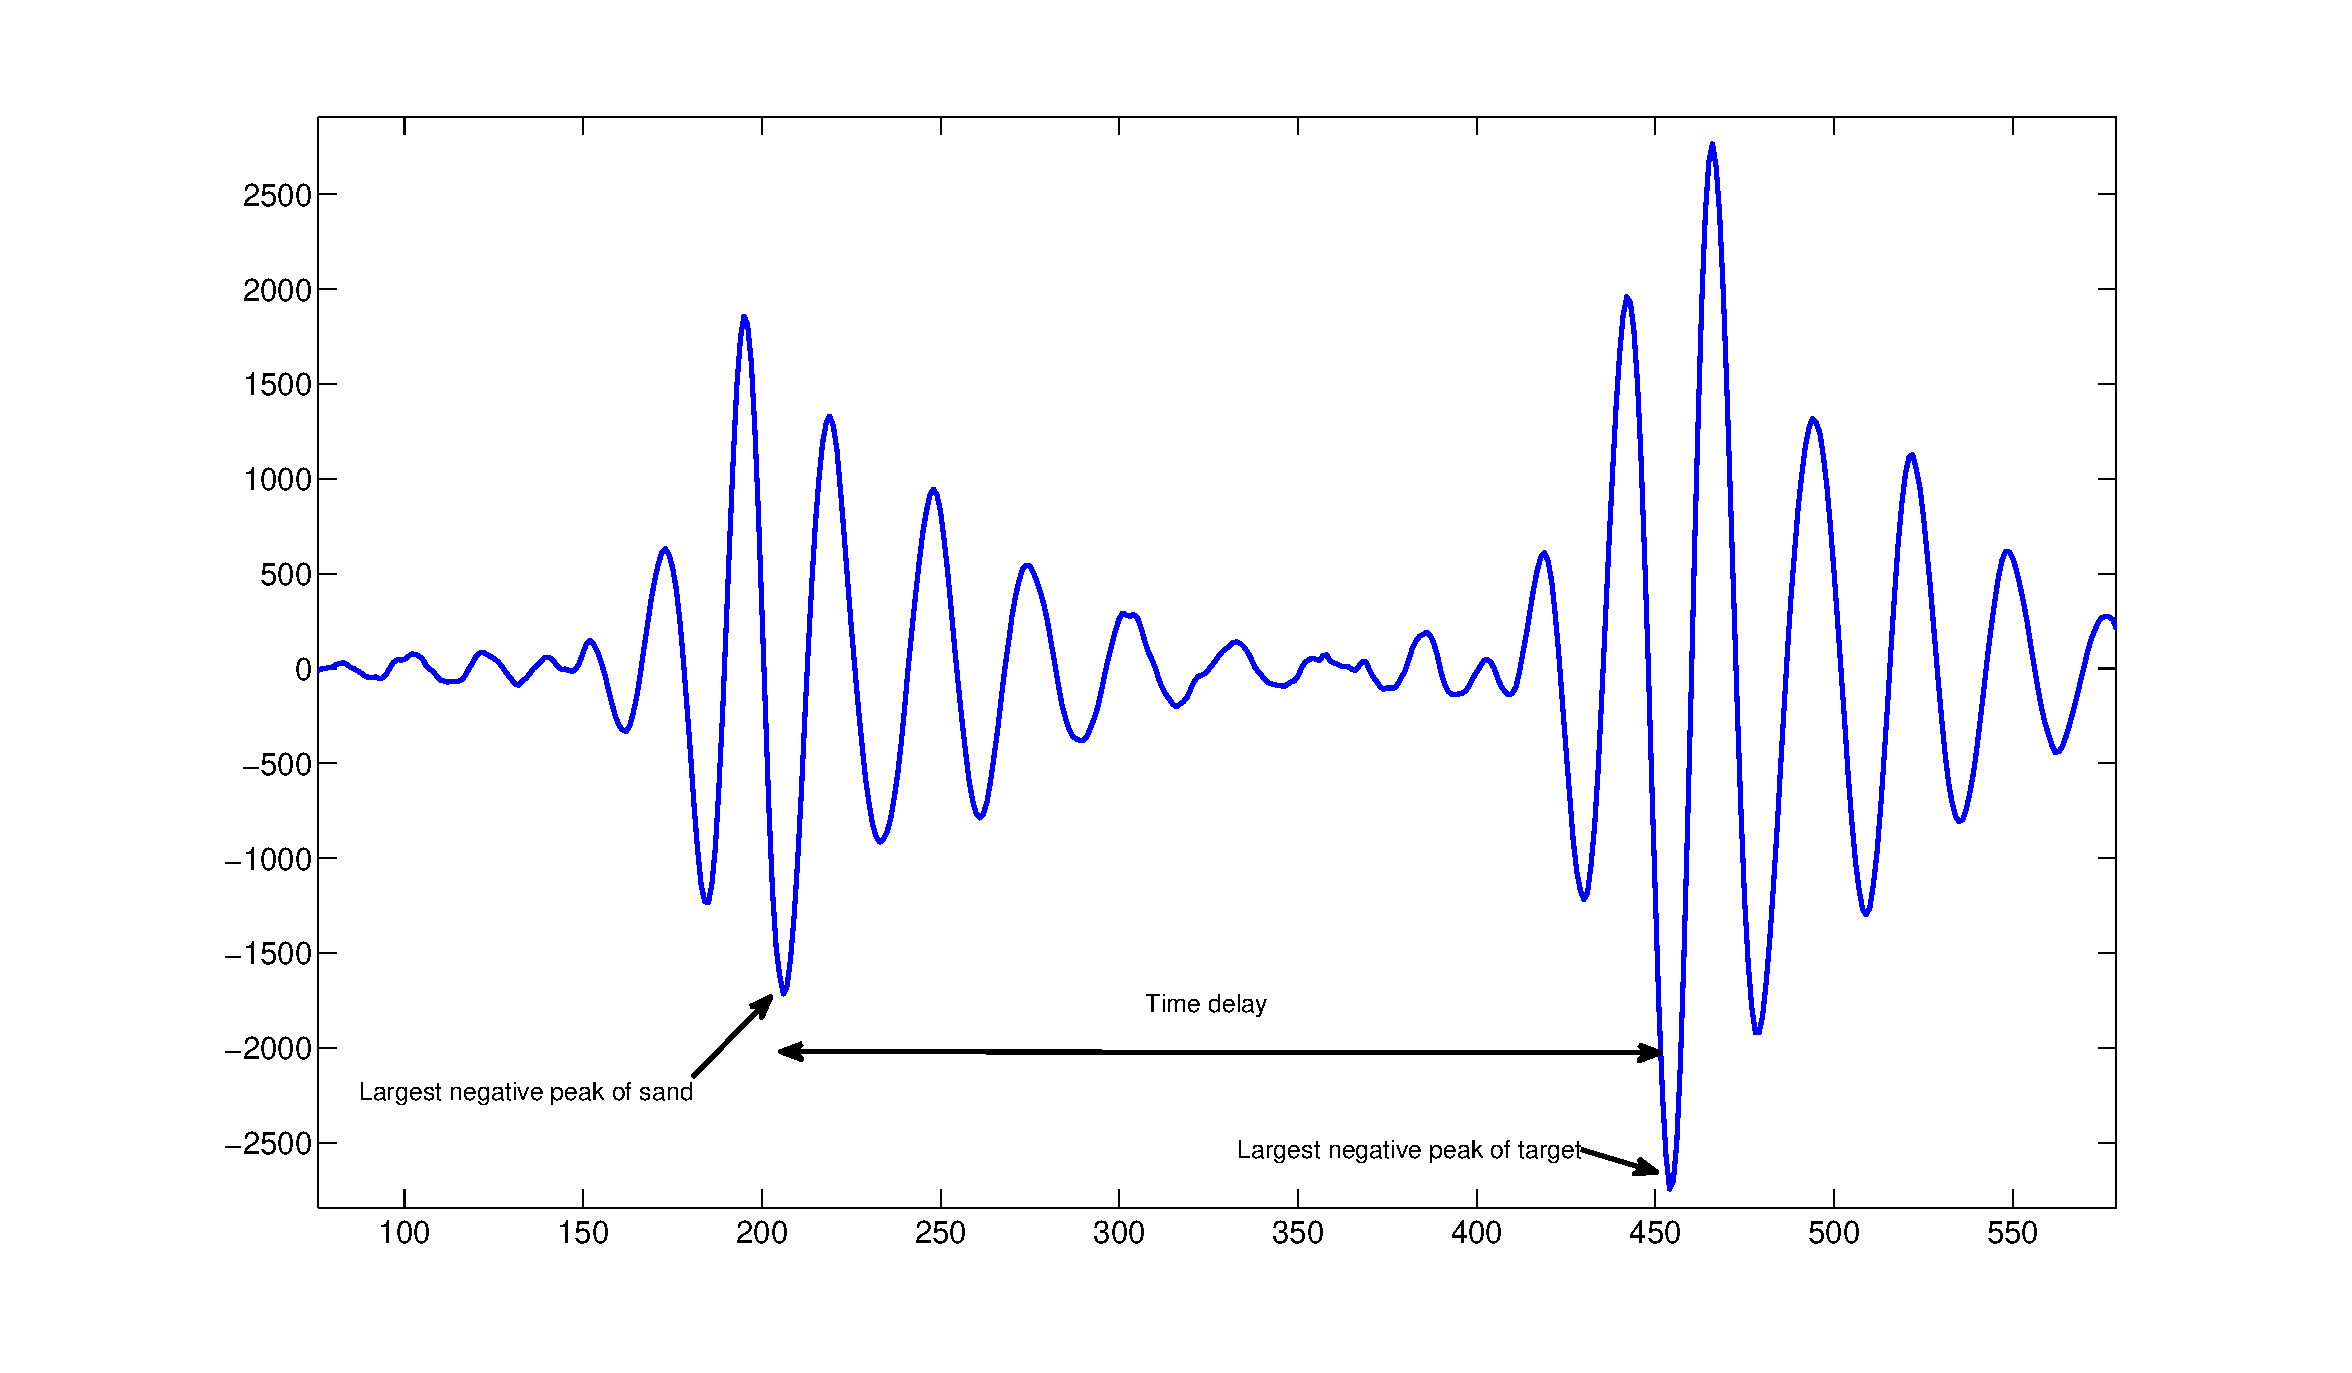
\includegraphics[width =0.9\textwidth]{figure/depth_estimate_1}
\caption{The largest negative peaks of the sand and the target for a metallic target buried at 14 cm. The distance between them is the time delay, which is used to determine the depth of burial. }
\label{fig:4.30}
\end{figure}



After running this step, which is step 6 in the code, the data should be double-checked to make sure that it works since the criterion used in the extraction of target's signal may be different for different experiments. 



\begin{figure}[tph]
\centering
\subfigure[A strong target]{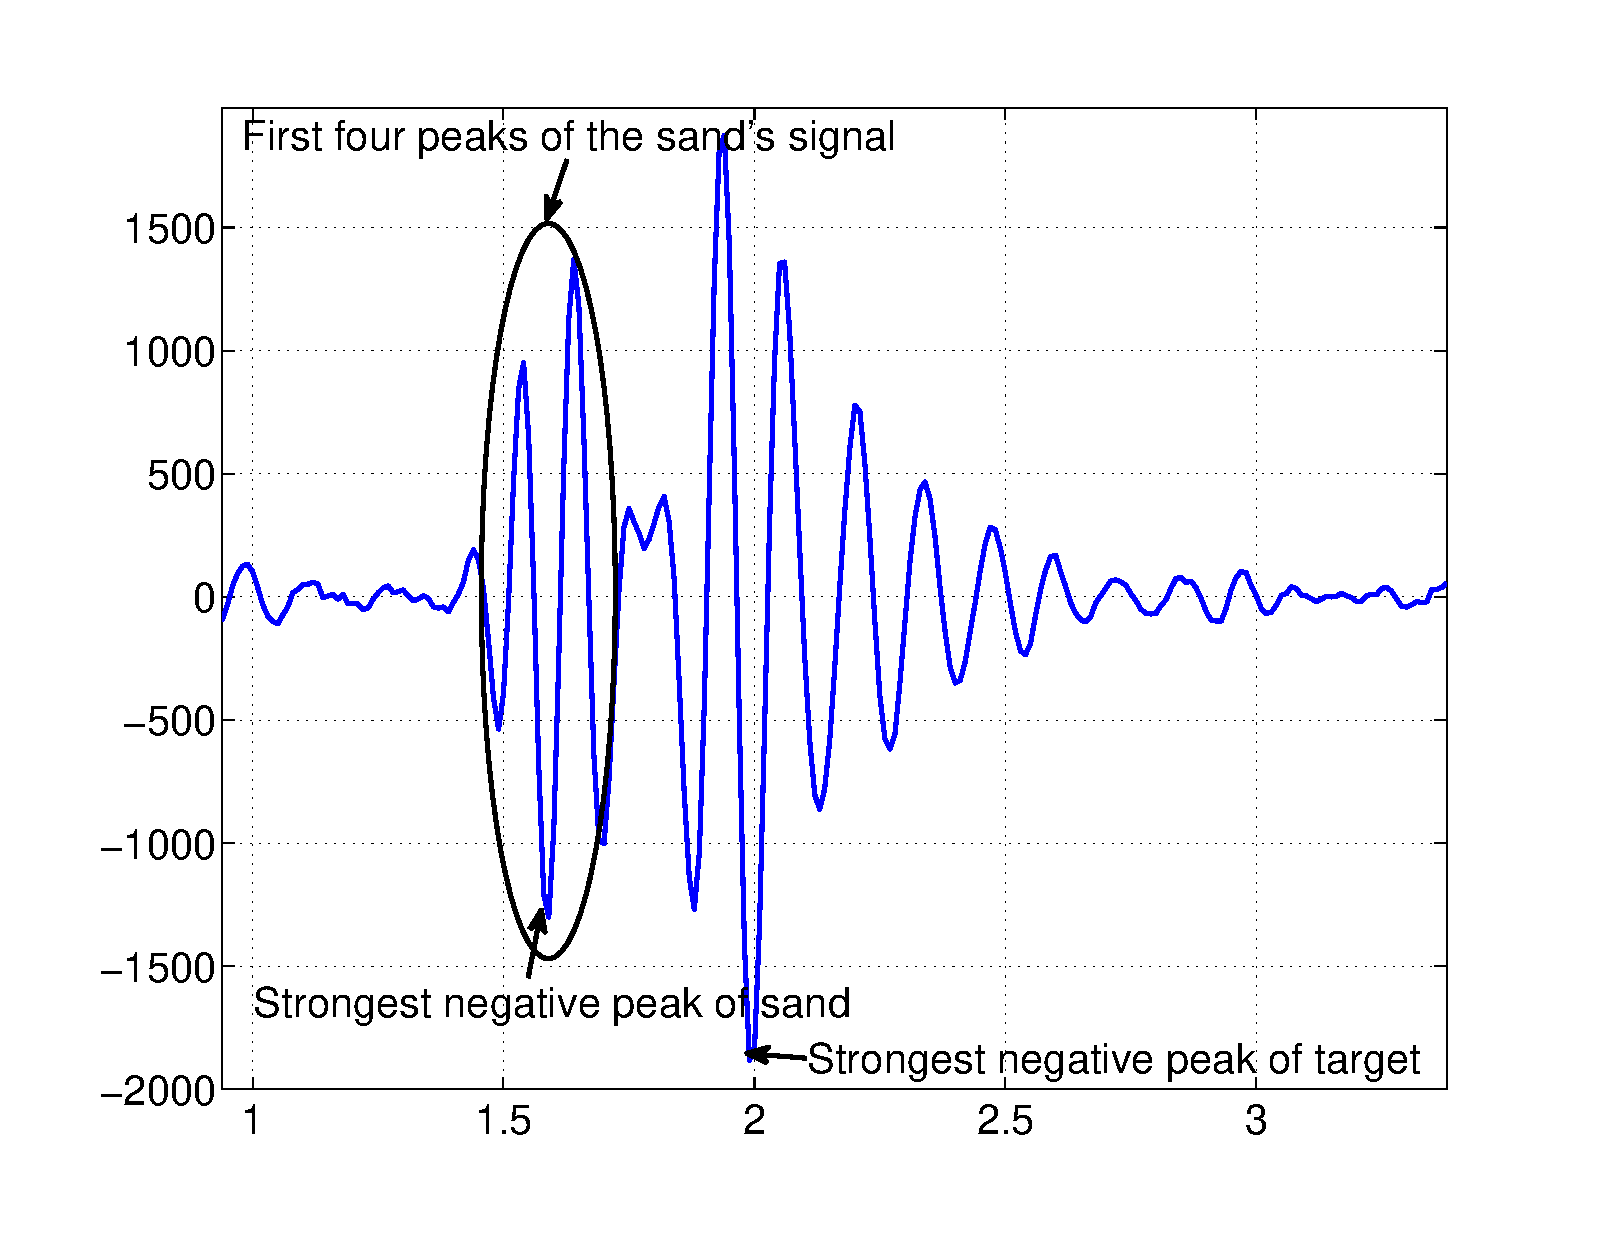
\includegraphics[width =
0.48\textwidth]{figure/Figure10_a2}} 
\subfigure[A weak
target]{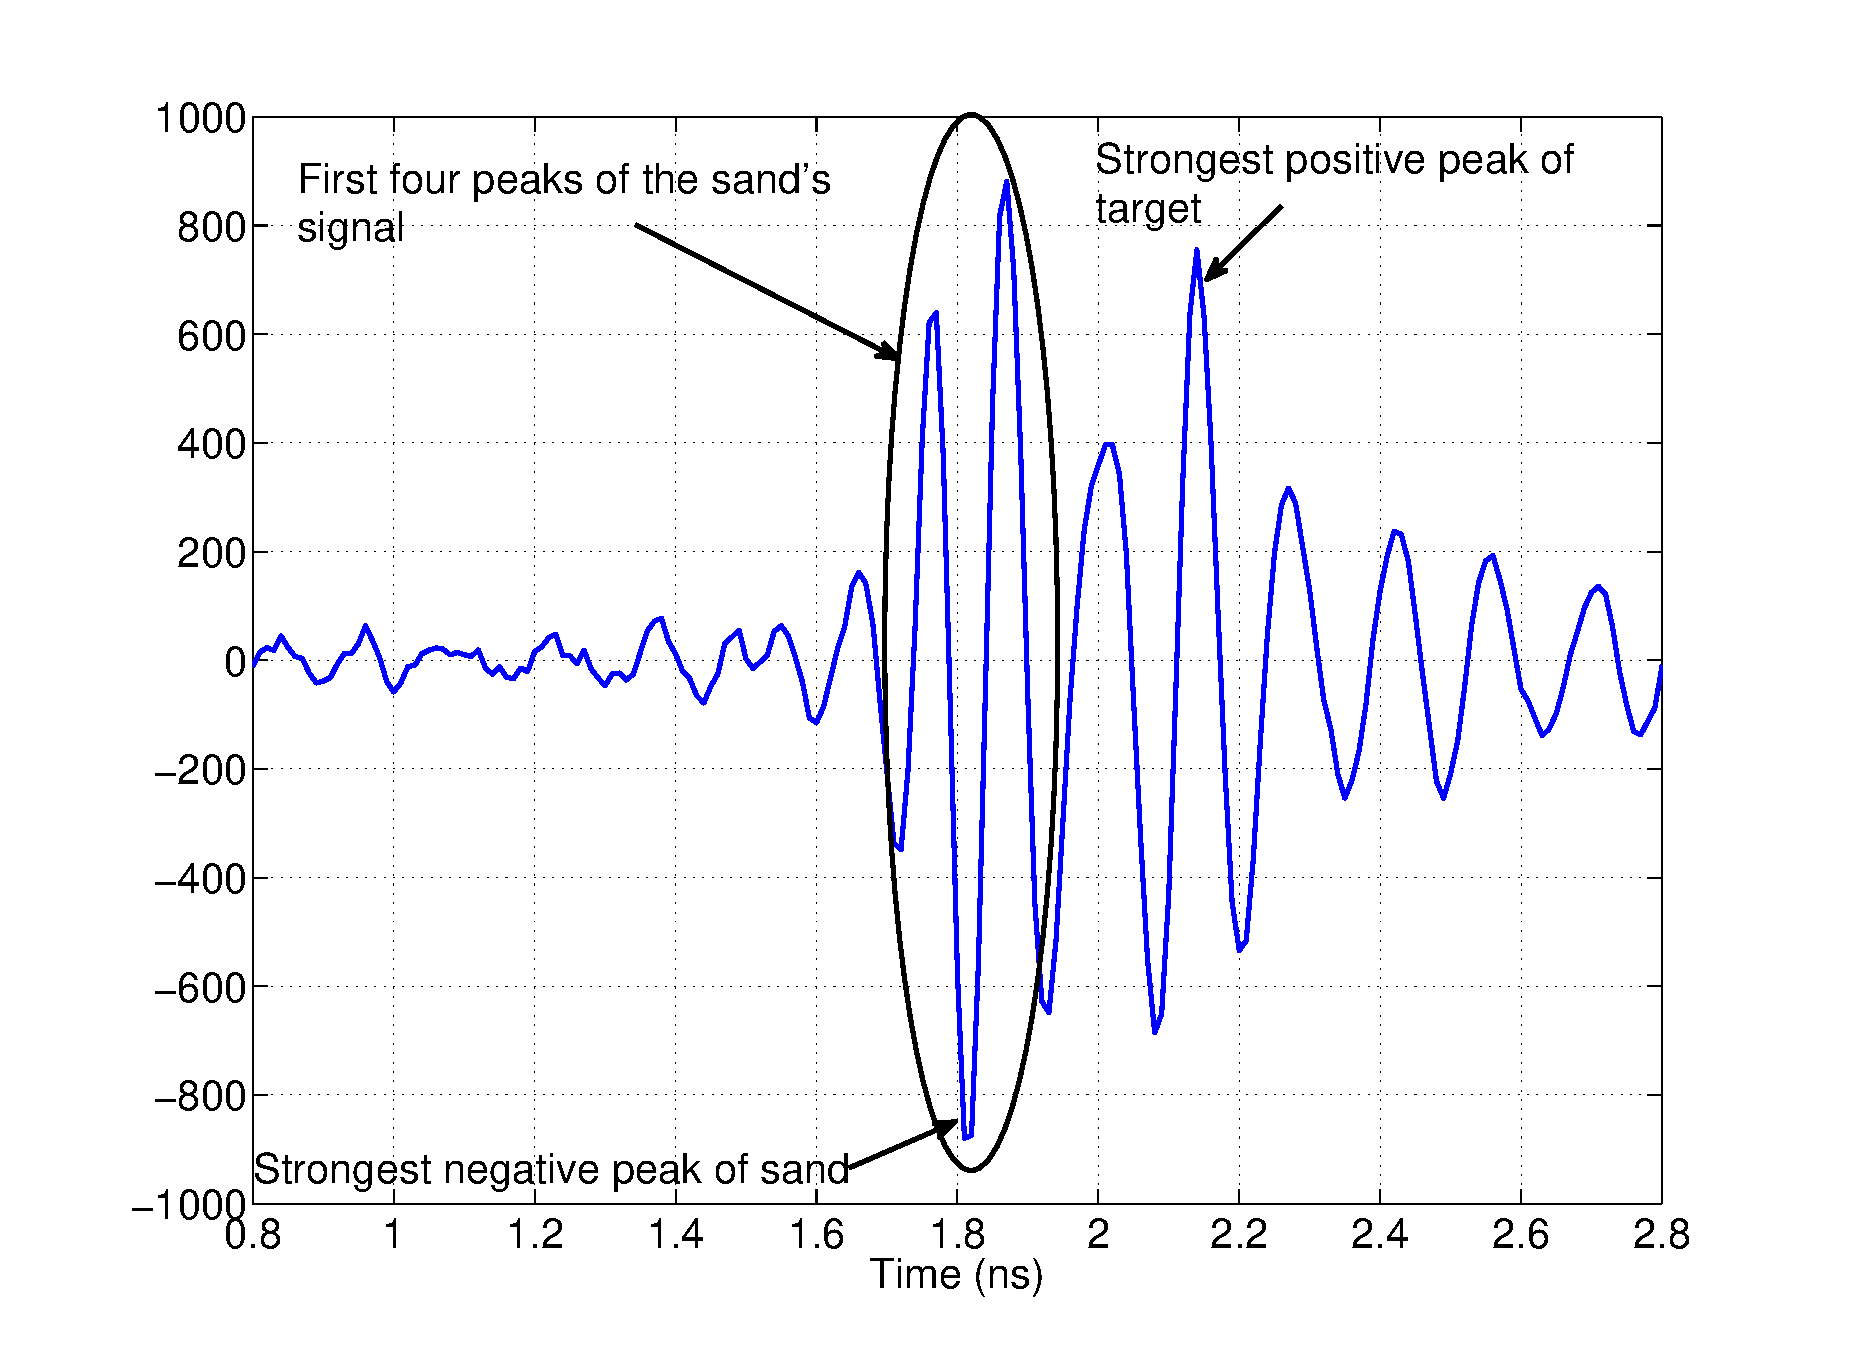
\includegraphics[width = 0.48\textwidth]{figure/Figure10_b2}}
\caption{One-dimensional propagated signals at the strongest detectors of
two targets: one strong target and one weak target. 
The signals consist of the reflection from the sand's surface followed by the
reflections from the targets.}
\label{fig:4.3}
\end{figure}





\subsubsection{Data scaling (calibration)}
Finally, since the amplitude of
the experimental signals are usually quite different
from the simulated ones, we scale the former to better match the latter in amplitude by multiplying the former by a certain factor, which we call  the
\emph{calibration factor}. The choice of this factor is based on the data of a known
target referred to as the \textit{calibrating object}. See \cite{TBKF:SISC2014} for details. 



\section{Frequency-dependent data}



\bibliographystyle{abbrv}
\bibliography{../../../publication-talks/bibliography/references_gca,../../../publication-talks/bibliography/references_full}

\end{document}

